% !TeX spellcheck = en_B
% !TeX encoding = UTF-8 %%%These comments just make you look like you know what you're doing
\documentclass[8pt]{beamer}  %%% Specifies the class, with 8pt font size

\usepackage[utf8]{inputenc}

\usetheme[block=fill,numbering=fraction,sectionpage=none,background=light]{metropolis}

\usepackage[english]{babel}
\usepackage{csquotes}       
\usepackage[T1]{fontenc}        
\usepackage{booktabs}
\usepackage{pgfgantt}
\usepackage{pifont}
\usepackage{adfbullets}
\usepackage{enumitem}
\usepackage{tikz}
\usepackage{lipsum}
\usepackage{amssymb}
\usepackage{amsfonts}
\usepackage{mathrsfs}
\usepackage{adjustbox}
\usepackage{varioref}
\usepackage{probsoln}
\usepackage{attachfile2}
\usepackage{pgfplots}
\pgfplotsset{compat=newest}
\graphicspath{{Graphics/}}
\usepackage{multirow,array}
\usepackage{colortbl}
\definecolor{aa}{RGB}{255, 124, 0}
\definecolor{cc}{RGB}{230, 230, 230}    
\usebackgroundtemplate{%
    \tikz[overlay,remember picture]{
        \node[scale=0.3,opacity=0.08,xshift=-8cm,yshift=+26.7cm] at (current page.south east){
            
\includegraphics{assets/img/marchio_unitrento_colore_it_202002.eps}
        }
    }
}

%% Indispensables

\usepackage{amsmath}
\usepackage{graphicx}

\usepackage{booktabs}
\newcommand{\ra}[1]{\renewcommand{\arraystretch}{#1}}

\usepackage{tabularx}

%% bibliography
\usepackage[backend=bibtex,style=verbose-trad2]{biblatex}
\bibliography{bibliography.bib}

%% listings
\usepackage{listings}
\usepackage{xcolor}

\colorlet{punct}{red!60!black}
\definecolor{background}{HTML}{EEEEEE}
\definecolor{delim}{RGB}{20,105,176}
\colorlet{field}{magenta!60!black}

\lstdefinelanguage{json}{
    basicstyle=\small\tt,
    numberstyle=\scriptsize,
    showstringspaces=false,
    breaklines=true,
    frame=none,
    literate=
      {,}{{{\color{punct}{,}}}}{1}
      {\{}{{{\color{delim}{\{}}}}{1}
      {\}}{{{\color{delim}{\}}}}}{1}
      {[}{{{\color{delim}{[}}}}{1}
      {]}{{{\color{delim}{]}}}}{1},
    string=[s]{"}{"},
    stringstyle=\color{field},
    comment=[l]{:},
    commentstyle=\color{black},
}

\usepackage{comment}
\usepackage{varwidth}

\newcommand{\mat}[4]{\left(\begin{array}{cc} #1 & #2 \\ #3 & #4 \\ \end{array}\right)}
\newcommand{\Q}{\mathbb{Q}}
\newcommand{\R}{\mathbb{R}}
\newcommand{\Z}{\mathbb{Z}}
\newcommand{\sol}[2][+]{
	\tikz[baseline]{\node[color=aa,fill=cc,rectangle,draw,anchor=base] {  {\onslide<#1->{#2}}  };}
}

\usetikzlibrary{positioning}
\usetikzlibrary{tikzmark}
\usetikzlibrary{shadings}
\usetikzlibrary{through}

\def\height{0.8cm}
\def\width{1.2cm}
\newcommand{\keynode}[6]{\node[minimum height=\height,minimum width=\width,draw,rectangle,color=aa,fill=cc] (#3) at (#1,#2) {};
	\node[rectangle,minimum height=\height/2,minimum width=\width,above,color=aa] at (#3) {#3};
	\node[draw,rectangle,minimum height=\height/2,minimum width=\width/3,below,color=aa,fill=cc,inner sep =0cm] at (#3) {\footnotesize#4};
	\node[draw,rectangle,minimum height=\height/2,minimum width=\width/3,below,xshift=\height/2,color=aa,fill=cc,inner sep=0cm] at (#3) {\footnotesize#5};
	\node[draw,rectangle,minimum height=\height/2,minimum width=\width/3,below,xshift=-\height/2,color=aa,fill=cc,inner sep=0cm] at (#3) {\footnotesize#6}; }

\newenvironment{gantt}[3]{\begin{ganttchart}[#1,bar height=.6,bar top shift=.2,title/.style=  {draw=none},y unit chart=0.6cm,y unit title = 0.6cm,include title in canvas=false,group/.append style={draw=black,dashed},bar/.append style={fill=aa},inline,hgrid=true,Float1/.style={bar/.append style={fill=none,dashed},bar height=.8,bar top shift=0.1}]{#2}{#3}}{\end{ganttchart}}

\newenvironment{nicetable}[1]{\setlength\arrayrulewidth{0.5mm}
			\arrayrulecolor{white}
			\begin{tabular}{#1}}{\end{tabular}}
		
\setlist[itemize,1]{label={\color{aa}\huge\adfbullet{36}}}
\setlist[itemize, 2]{label={\color{aa}\large\adfbullet{36}}}

\newcommand\reshist{}
\def\reshist(#1)#2(#3)#4(#5)%
{\draw (axis cs:#1) rectangle (axis cs:#3) node [midway] {#5};}

\usepackage[
    % hidelinks,
    % colorlinks=true,
]{hyperref} % importare per ultimo

\hypersetup{
    colorlinks = true,
    linkbordercolor = {white}, % rettangoli attorno ai link
    linkcolor = {},     % toc. {} significa nero
    urlcolor = {teal},  % link
    citecolor = {teal}, % bibliografia
}

\usepackage[capitalize, nameinlink, noabbrev]{cleveref} %%%adds the general preamble

%%%Title and subtitle
\title{Studying the emotional impact of the Covid-19 pandemic using social media}
\subtitle{Bachelor Degree Thesis Presentation, \textattachfile{alghisi_simone_slides_laurea_aa_2020_2021.tex}{(TeX)}} %%%This embeds the tikz source code into the resulting pdf...
\author[author1]{Simone Alghisi\\[1.5mm]{\small Supervisor: Alberto Montresor}\\[1.5mm]{\small Co-Supervisors: Cristian Consonni, David Laniado}\\[1.5mm]}
\institute{Università degli Studi di Trento}
\date[\today]{\today}

\begin{document}

\begin{frame}[plain,noframenumbering]
    \titlepage
\end{frame}

\setcounter{tocdepth}{1}

\begin{frame}[plain,noframenumbering]
    \frametitle{Contents}
    \tableofcontents
\end{frame}

\setlength{\abovedisplayskip}{0pt}
\setlength{\belowdisplayskip}{0pt}
\setlength{\abovedisplayshortskip}{0pt}
\setlength{\belowdisplayshortskip}{0pt}  %%%Compresses math

\section{Introduction}
\begin{frame}{Introduction to the problem}

    The project consisted in an \textbf{analysis of emotions as emerging from Twitter messages} during the pandemic.
    
    \begin{figure}[H]
    	\centering
    	
\includegraphics[scale=.35]{assets/img/john_doe_tweet.png}
    	\caption{An example of a tweet.}
    	\label{fig:tweet-example}
    \end{figure}
    
    This could allow us to contrast the emotional reaction with the evolution of contagions and deaths, and with the different lockdown and de-escalation stages, in different areas.

\end{frame}

\begin{frame}{Emotion detection}

    Also called emotion recognition, is the \textbf{process of identifying human emotions}~\autocite{enwiki:1023798177}. To solve this task, it is possible to use lexicon-based techniques, where each word is assigned to a set of zero or more emotions/sentiments.

    \begin{figure}[H]
    	\centering
    	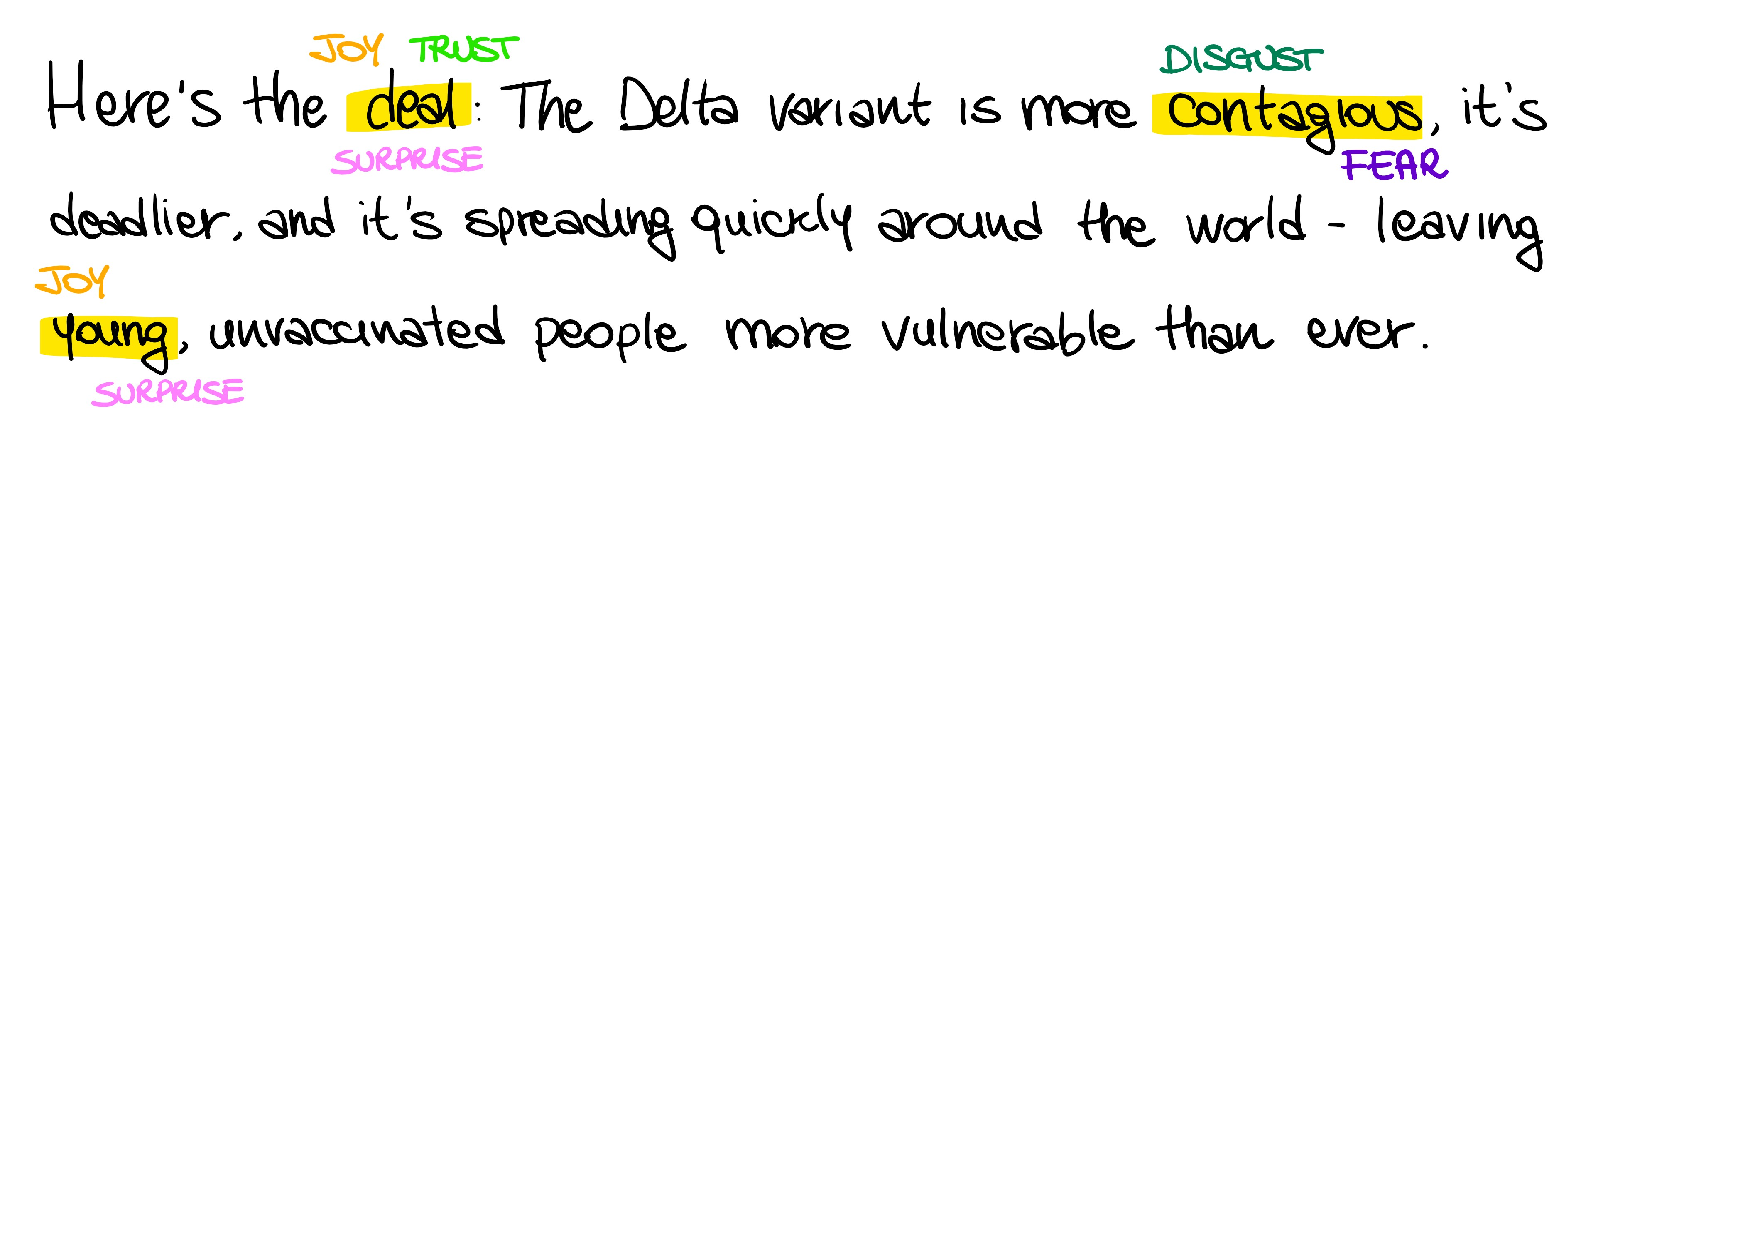
\includegraphics[scale=.45,trim= 0 700 0 30, clip]{assets/img/emotion_detection_example.pdf}
    	\caption{Emotion detection for a particular sentence.}
    	\label{fig:emotion-detection-example}
    \end{figure}

\end{frame}

\begin{frame}{Contributions}

    In general, my contribution to the research mostly regarded:
    
    \begin{itemize}
    	\item retrieving and organizing the data
    	\item processing the tweets to understand users' emotions
    	\item plotting graphics in order to visualize more clearly the results
    	\item normalizing the results obtained to compare different emotions or categories
    	\item inferring demographic information about the users
    	\item geocoding the location of the user
    \end{itemize}
    
    Furthermore, I am particularly proud of my personal contribution to improve m3inference. In practice, I opened a pull request on GitHub to solve some issues while downloading images from Twitter.

\end{frame}

\section{Data collection}

\begin{frame}{Dataset description and stats}

	The \textbf{echen102/COVID-19-TweetIDs} GitHub repository contains an ongoing collection of tweet IDs starting on January 28th, 2020~\autocite{chen2020tracking}.
	
	\begin{table}[H]
        \centering
        \ra{1.2}
        \begin{tabular}{lr}
            Number of files & 10 402
            \\
            Number of identified languages & 65
            \\
            Number of tweets & 1 055 843 481
            \\
            Number of unique tweets (no retweets) & 323 504 667
            \\
            Dataset compressed size & 865 GB
            \\
            Dataset estimated uncompressed size & 6.252 TB
        \end{tabular}
        \caption{Dataset general statistics}
        \label{tab:dataset-stats}
    \end{table}

\end{frame}

\begin{frame}[fragile]{Tweet Structure}

    We decided to analyze the tweets \textbf{from January 2020 to March 2021}, keeping only the most relevant information.
	
    \begin{lstlisting}[language=json, caption={Final json object for a tweet}, captionpos=b, label={lst:tweet_json}]
{
  "id": 1307025659294674945,
  "full_text": "Here's an article that highlights the updates...",
  "lang": "en",
  "created_at": "Fri Sep 18 18:36:15 +0000 2020",
  "retweet_count": 11,
  "favorite_count": 70,
  "user": {
    "id": 2244994945,
    "id_str": "2244994945",
    "screen_name": "TwitterDev",
    "name": "Twitter Dev",
    "description": "The voice of the #TwitterDev team and your official...",
    "location": "127.0.0.1",
    "followers_count": 513958,
    "statuses_count": 3635,
    "default_profile_image": false,
    "profile_image_url_https": "https:\/\/pbs.twimg.com\/profile_images\/1283786620521652229\/lEODkLTh_normal.jpg"
  }
}
    \end{lstlisting}
	
\end{frame}

\section{Methods}

\begin{frame}{EmoLex \& LIWC}

    We used
    
    \begin{itemize}
        \item \textbf{EmoLex}, a list of English words and their associations with \textbf{eight basic emotions} (anger, fear, anticipation, trust, surprise, sadness, joy, and disgust) and \textbf{two sentiments} (negative and positive)~\autocite{ncrwebsite}, to detect the emotions
        \item \textbf{LIWC}, a widely used computerized text analysis program that outputs the percentage of words in a given text that falls into one or more \textbf{linguistic, psychological, and topical categories}~\autocite{enwiki:1023542720}, to validate the results
    \end{itemize}

\end{frame}

\begin{frame}{Emotion detection metrics}

    To correctly \textbf{detect the users' emotions}, we decided to follow one of the approaches discussed by Aiello et al.~\autocite{aiello2020epidemic}
	
	\begin{itemize}
    	\item emotions in a binary way (e.g. whether at given time the user expressed joy or not)
    	\item users over tweets (e.g. the number of unique users, instead of tweets, that expressed joy at a given time)
    \end{itemize}
	
    \begin{definition}
    \label{def:user-emotions}
    	Given \(U_e(t)\), the number of distinct users that expressed emotion \(e\) at time \(t\) in a tweet, and \(U(t)\), the number of distinct users that tweeted at time \(t\),
    	
    	\[f_e(t) = \frac{U_e(t)}{U(t)}\]
    	
    	is the proportion of users that expressed emotion \(e\) at time \(t\).	
    \end{definition}

\end{frame}

\begin{frame}{Emotion detection over time}

    We decided to analyze for the whole time frame the emotions of different set of users. In particular we grouped them
    
    \begin{itemize}
        \item by \textbf{language} (e.g. Catalan, Italian, English, Spanish, \ldots)
        \item by \textbf{gender} (male or female)
        \item by \textbf{age} (\(\geq 40\) or \(< 40\))
        \item by \textbf{location} (e.g. per state, country, county, \ldots)
    \end{itemize}

\end{frame}

\begin{frame}{Data Normalization}

    The issue is that the \textbf{emotions course are not easily comparable}. For this reason, it was decided to normalize the data using the \textit{z-score}.
	
    \begin{definition}
    \label{def:z-score}
    	Given \(f_e(t)\) and the period of time \([0,T]\),
    	
    	\[z_e(t) = \frac{f_e(t) - \mu_{[0,T]}(f_e)}{\sigma_{[0,T]}(f_e)}\]
    	
    	\[\text{where } \mu_{[0,T]}(f_e) = \frac{1}{\mid T \mid} \sum_{t =0}^{T} f_e(t) \text{, and } \sigma_{[0,T]}(f_e) = \sqrt{\frac{1}{\mid T \mid} \sum_{t = 0}^{T} \left( f_e(t) - \mu_{[0,T]}(f_e) \right)^2 }\] 
    \end{definition}

\end{frame}

\begin{frame}[fragile]{Users inference}

	To infer data about the users, we used m3inference, a \textbf{deep learning system for demographic inference} (gender, age, and person/organization) available on Python~\autocite{wang2019demographic}.
	
\begin{lstlisting}[language=json, caption={Json object returned by m3inference}, captionpos=b, label={lst:m3inference-prediction}]
{
  "gender": {
    "male": 0.8758, 
    "female": 0.1242
  }, 
  "age": {
    "<=18": 0.0053, 
    "19-29": 0.0363, 
    "30-39": 0.9239, 
    ">=40": 0.0346
  }, 
  "org": {
    "non-org": 0.9965, 
    "is-org": 0.0035
  }
}
\end{lstlisting}
	
\end{frame}

\begin{frame}[fragile]{Geocoding}
    
    To link users to a specific place, we need to perform \textbf{address geocoding}, the process of taking a text-based description of a location and returning its geographic coordinates.
    
    For this project, we decided to use \textbf{OpenStreetMap (OSM)} and the data made available by this particular service~\autocite{osm}.
    
\begin{lstlisting}[language=json, caption={Json object returned by Geopy given “Milano, Lombardia” as input}, captionpos=b, label={lst:nominatim-geocode}]
{
  "place_id": 317098601, 
  "licence": "Data \u00a9 OpenStreetMap contributors, ODbL 1.0. https://osm.org/copyright",
  "boundingbox": ["45.3867381", "45.5358482", "9.0408867", "9.2781103"], 
  "lat": "45.4668", 
  "lon": "9.1905", 
  "display_name": "Milano, Lombardia, Italia",
  "address": {
    "city": "Milano", 
    "county": "Milano",
    "state": "Lombardia", 
    "country": "Italia", 
    "country_code": "it"
  }
}
\end{lstlisting}
    
\end{frame}

\section{Results and discussion}

\begin{frame}{Emotions in the English tweets}

    \begin{figure}[H]
    	\centering
    	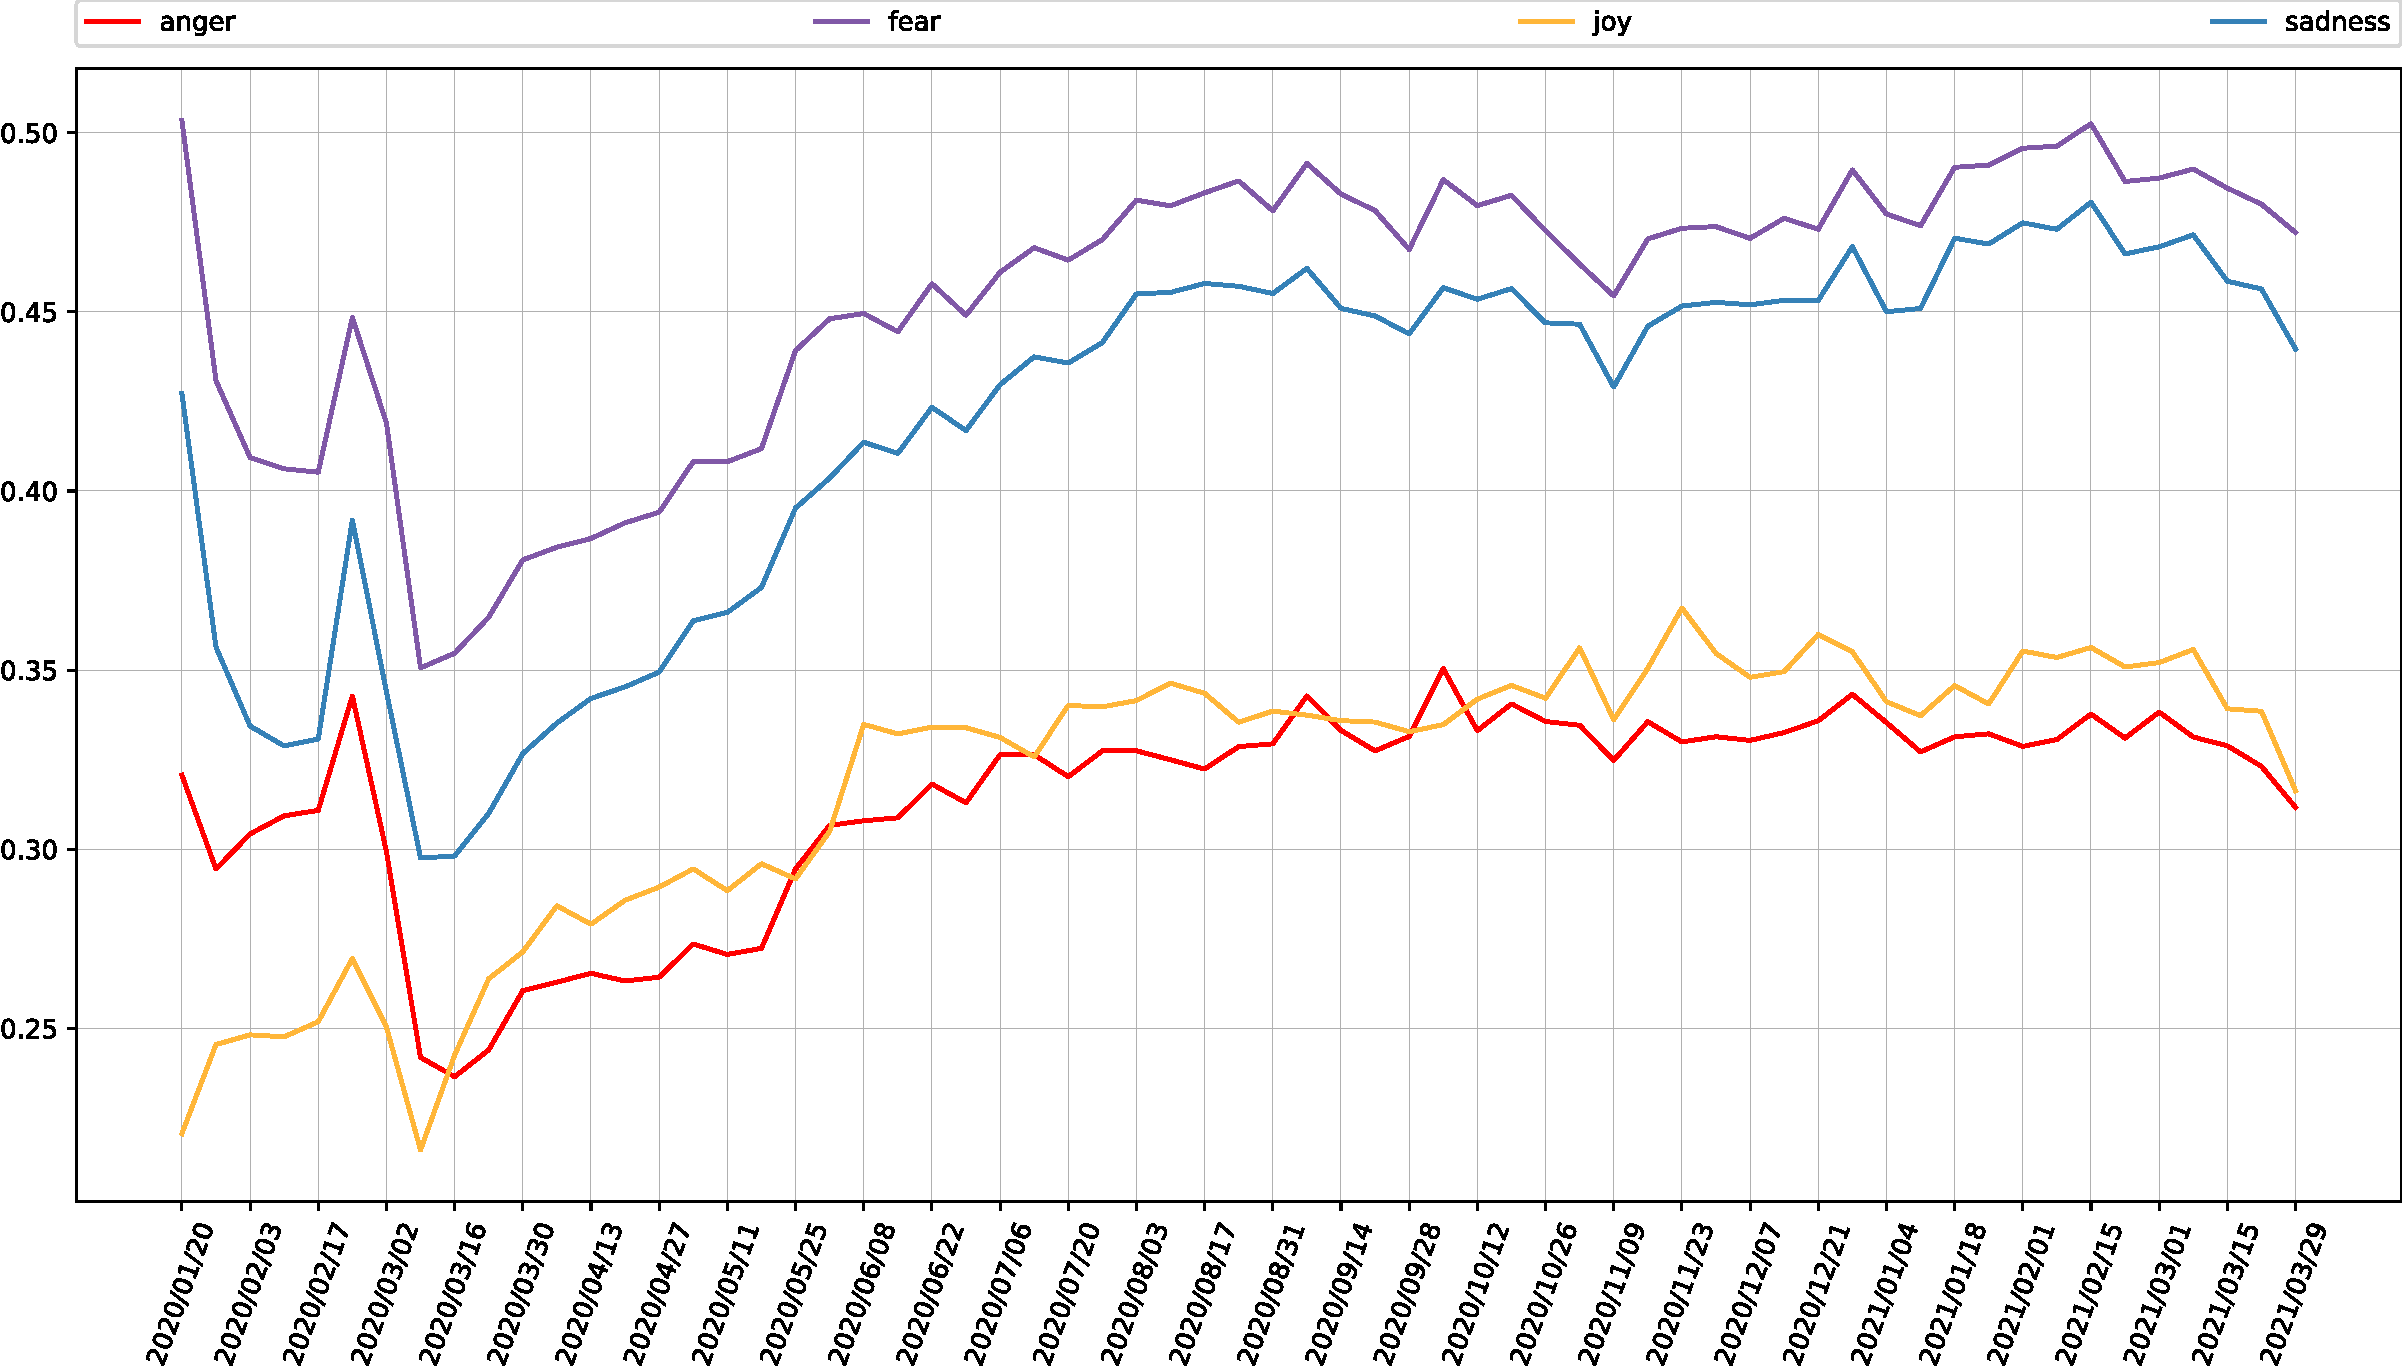
\includegraphics[scale=.25]{assets/img/en_4_emotions.svg.pdf}
    	\caption{Proportion of weekly users per emotion in the English tweets}
    	\label{fig:en-4-emotions}
    \end{figure}
    
\end{frame}

\begin{frame}{Normalized emotions in the English tweets}

    \begin{figure}[H]
    	\centering
    	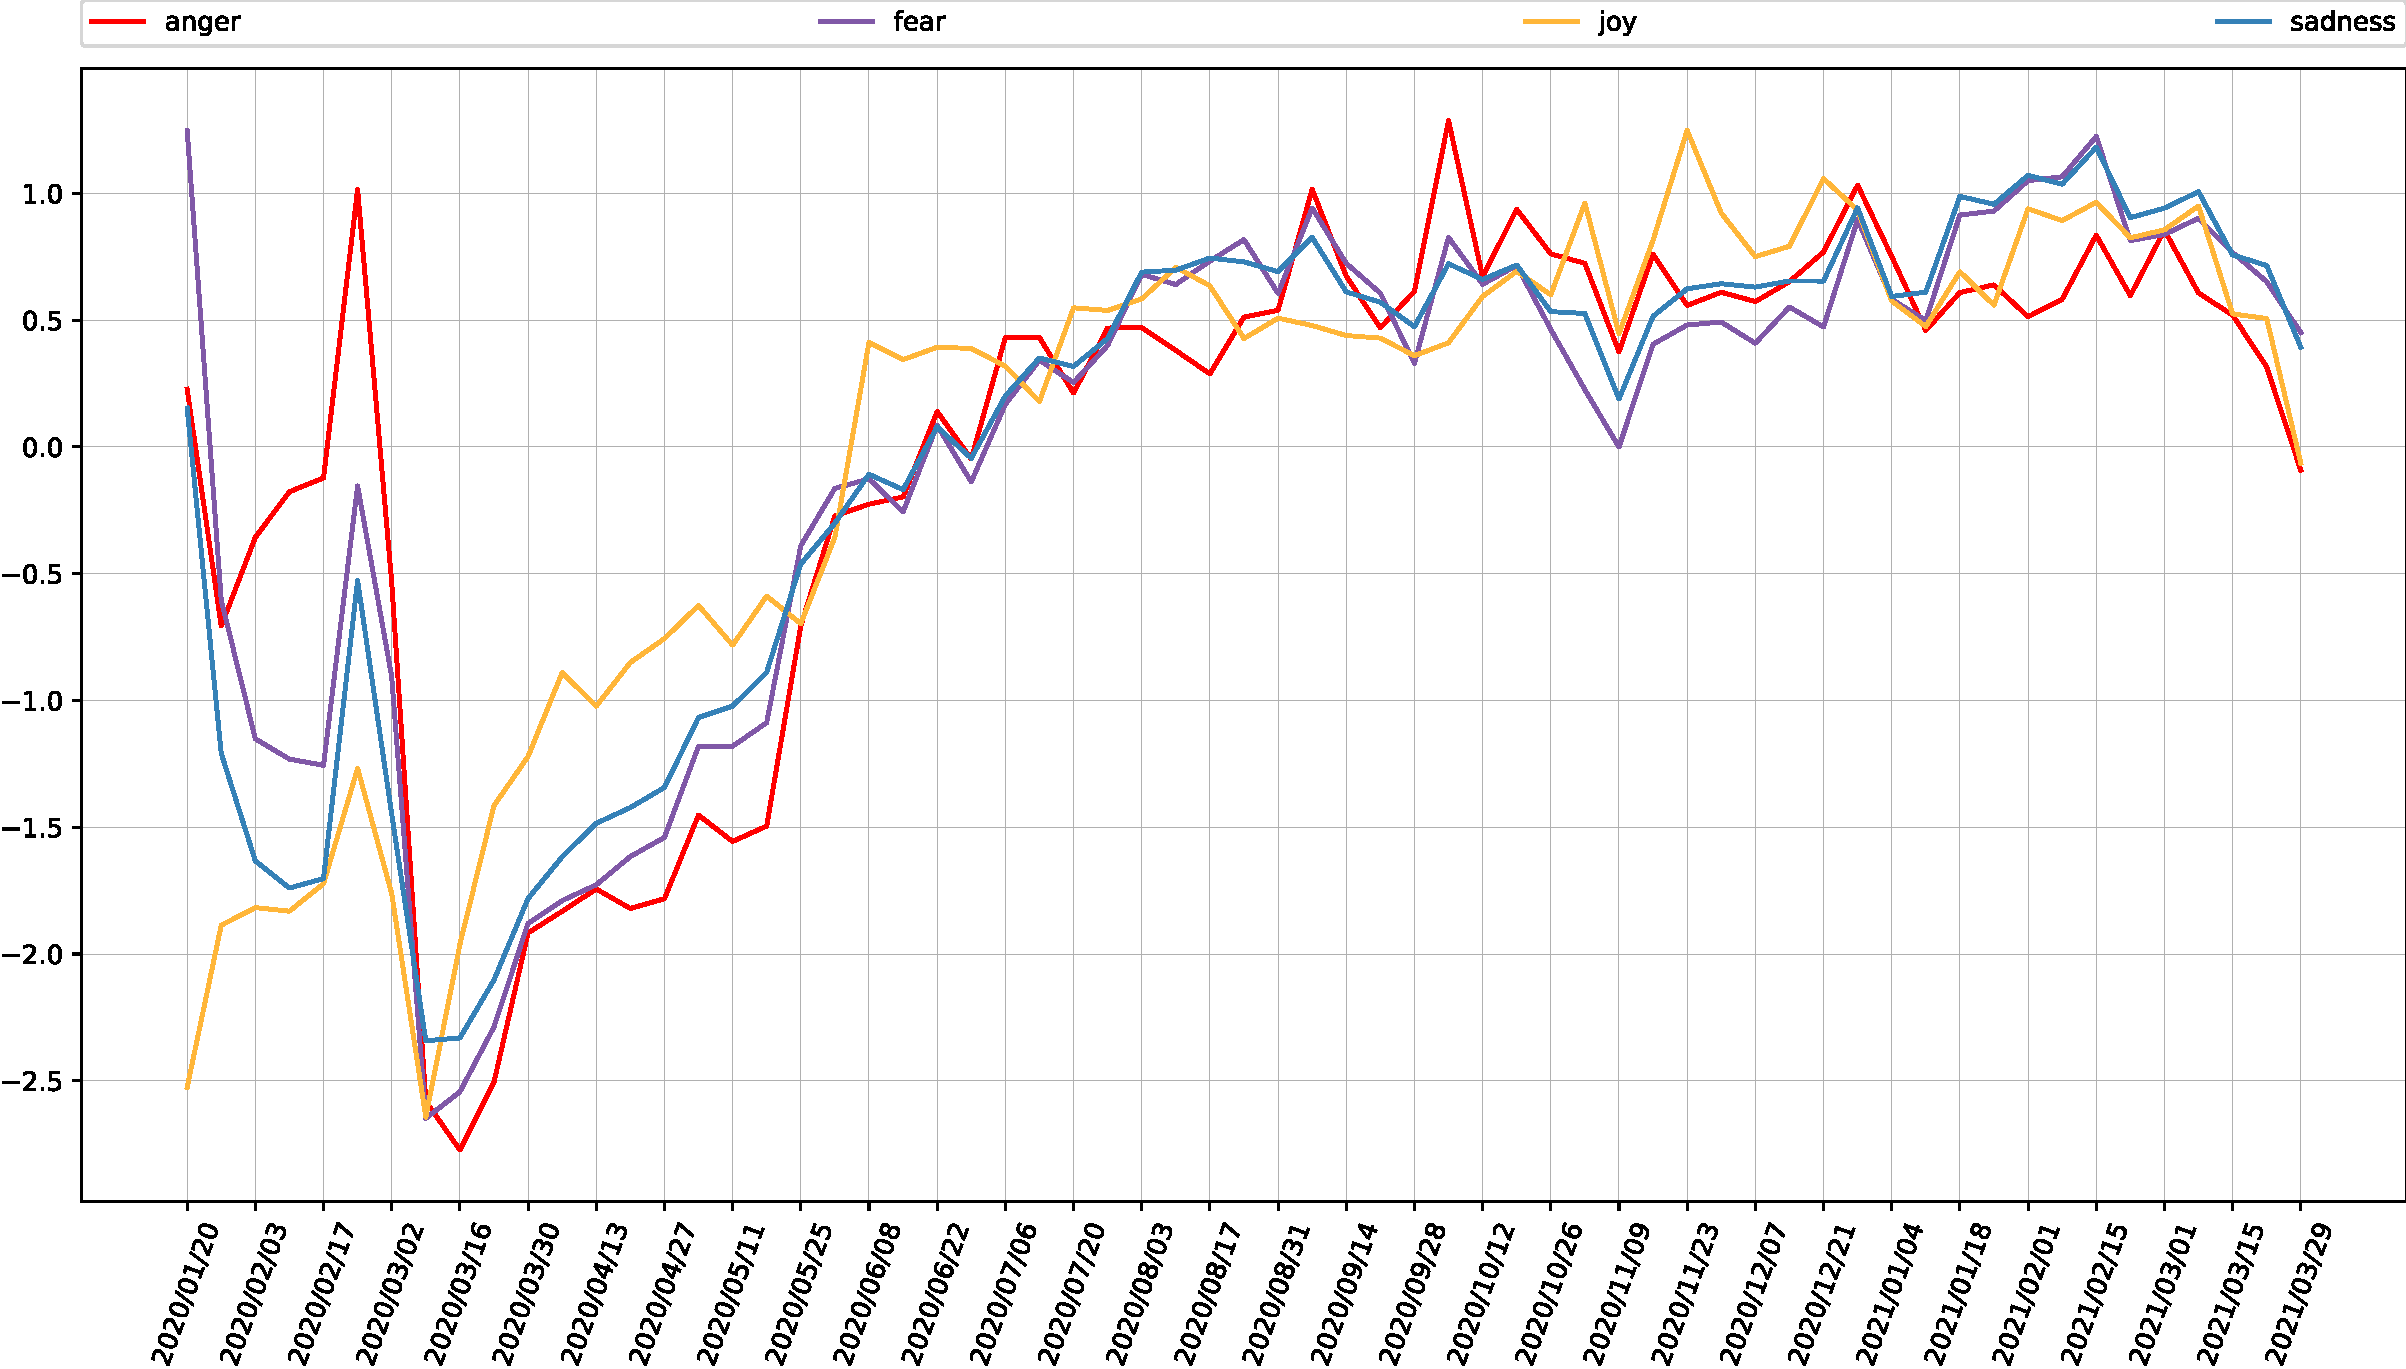
\includegraphics[scale=.25]{assets/img/en_4_emotions_standardized.svg.pdf}
    	\caption{Z-score of weekly users per emotion in the English tweets}
    	\label{fig:en-4-emotions-std}
    \end{figure}
    
\end{frame}

\begin{frame}{Emotions expressed by men/women in the English tweets}

    The dotted gray line represents the proportion of users that, independently from the category they belong to, expressed a certain emotion on a given week.

    \begin{figure}[H]
	    \centering
    	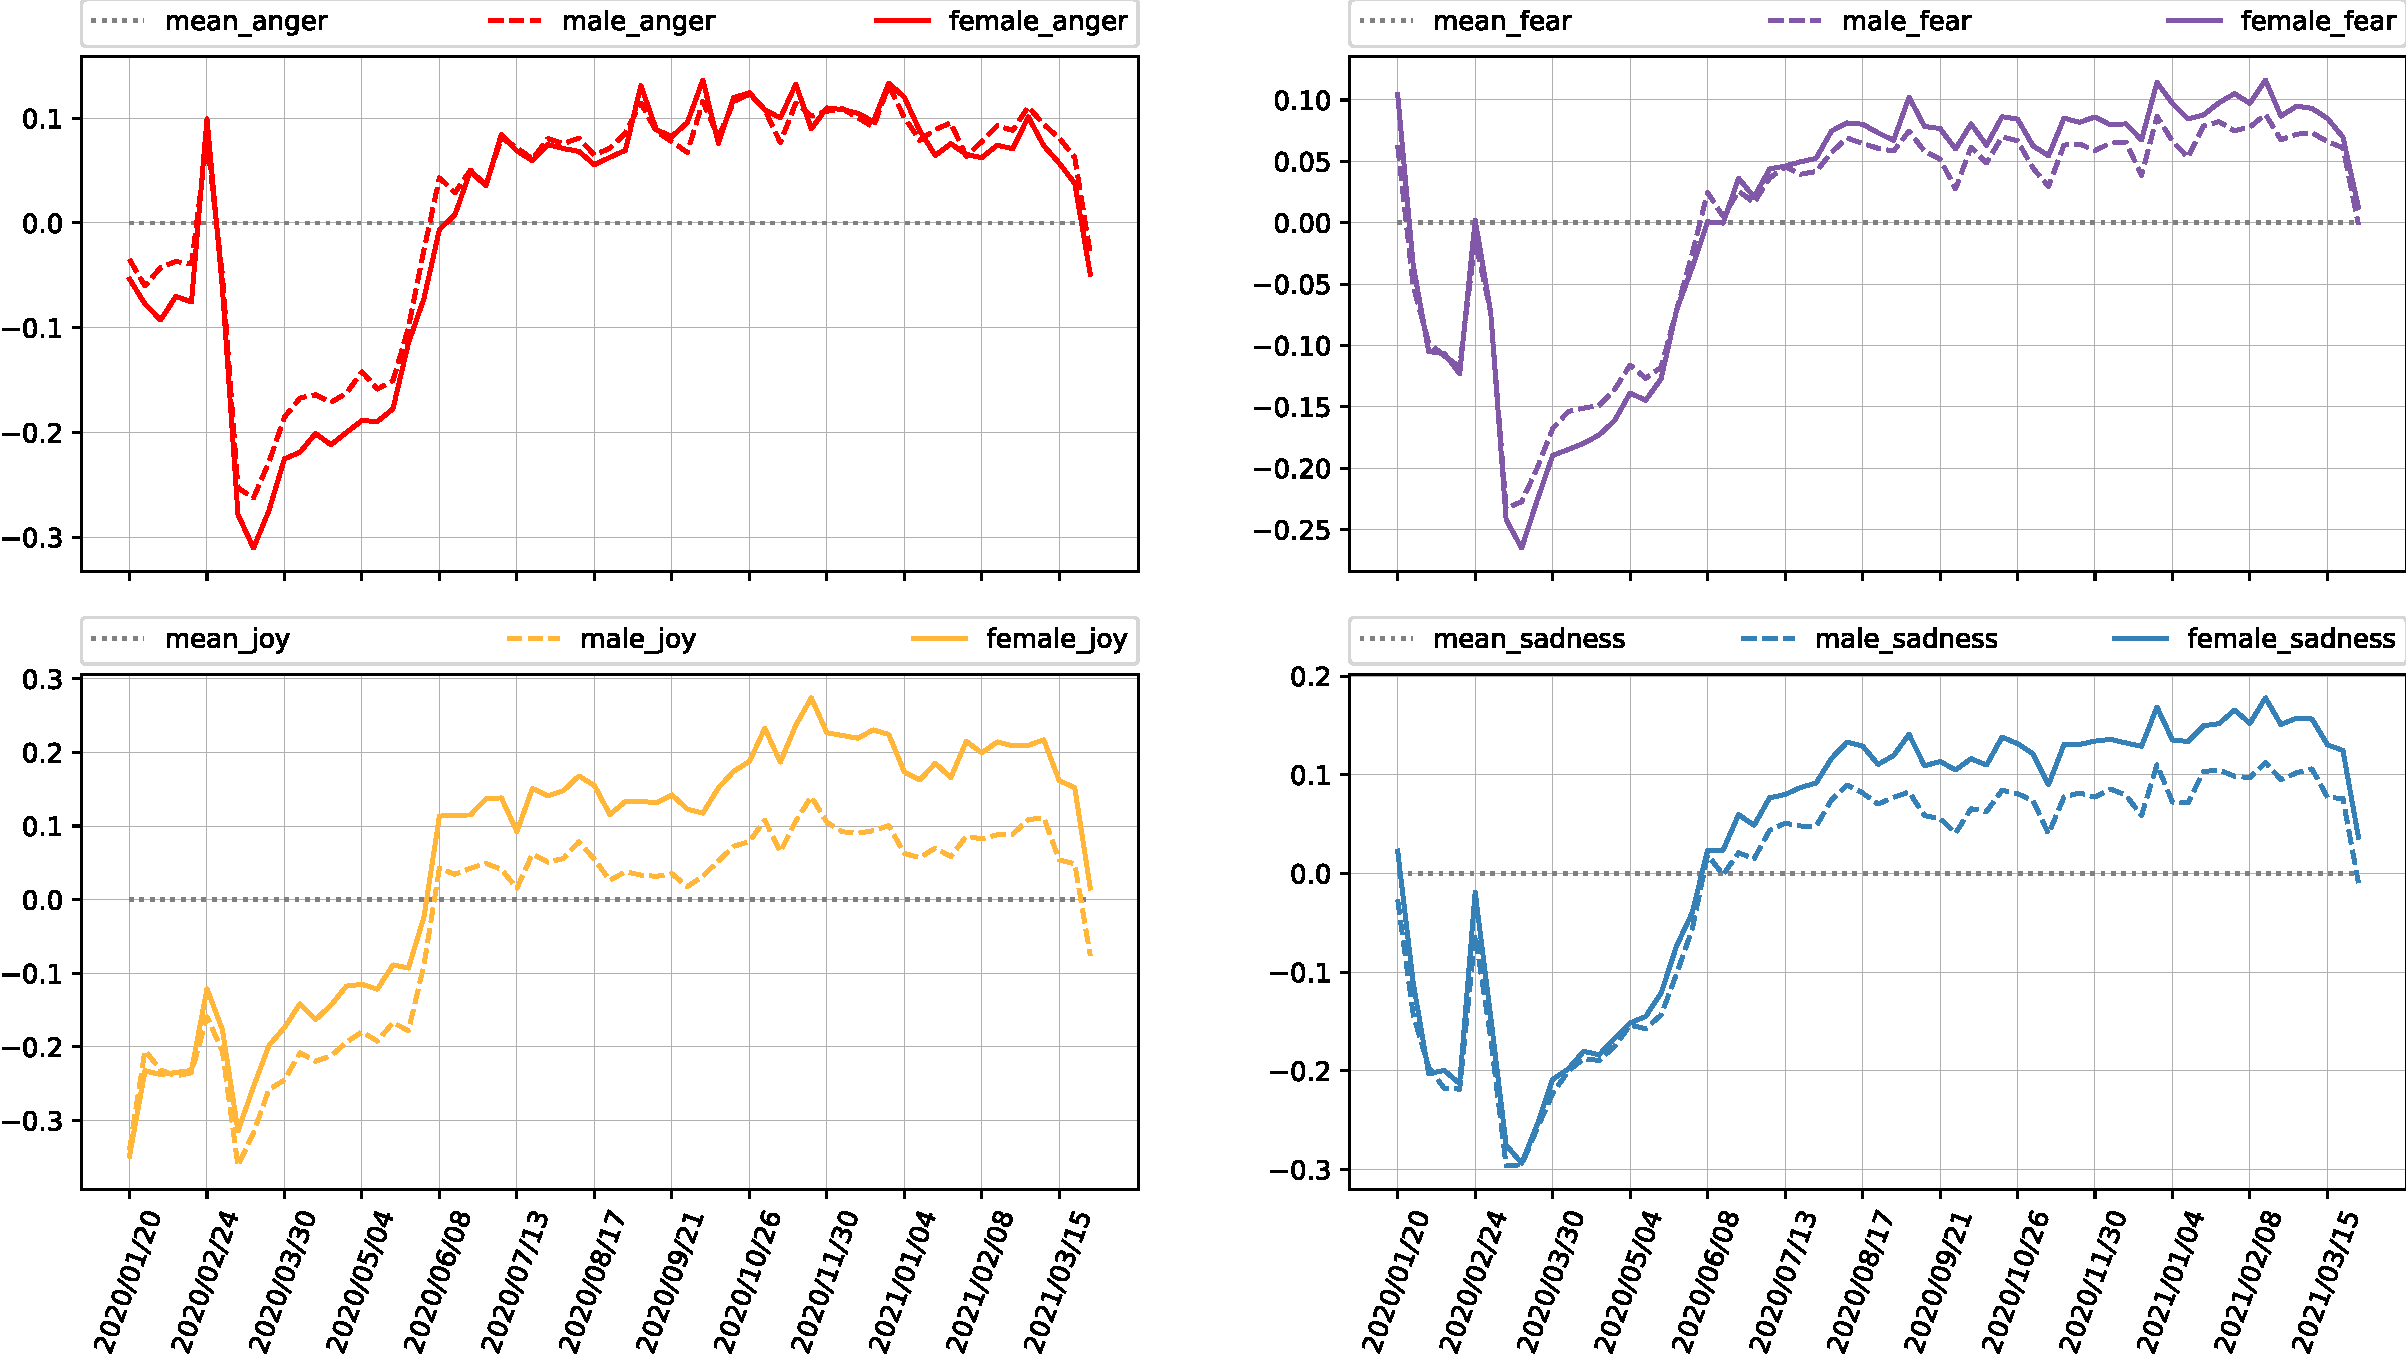
\includegraphics[scale=.22]{assets/img/en_4_emotions_per_category_over_mean_subplot_1.svg.pdf}
    	\caption{Men/Women expressing the weekly proportion of a particular emotion w.r.t. the average value among all users}
    	\label{fig:en-4-emotions-per-category-course-mean-1}
    \end{figure}
    
\end{frame}

\begin{frame}{Emotions expressed per age in the English tweets}

    \begin{figure}[H]
	    \centering
    	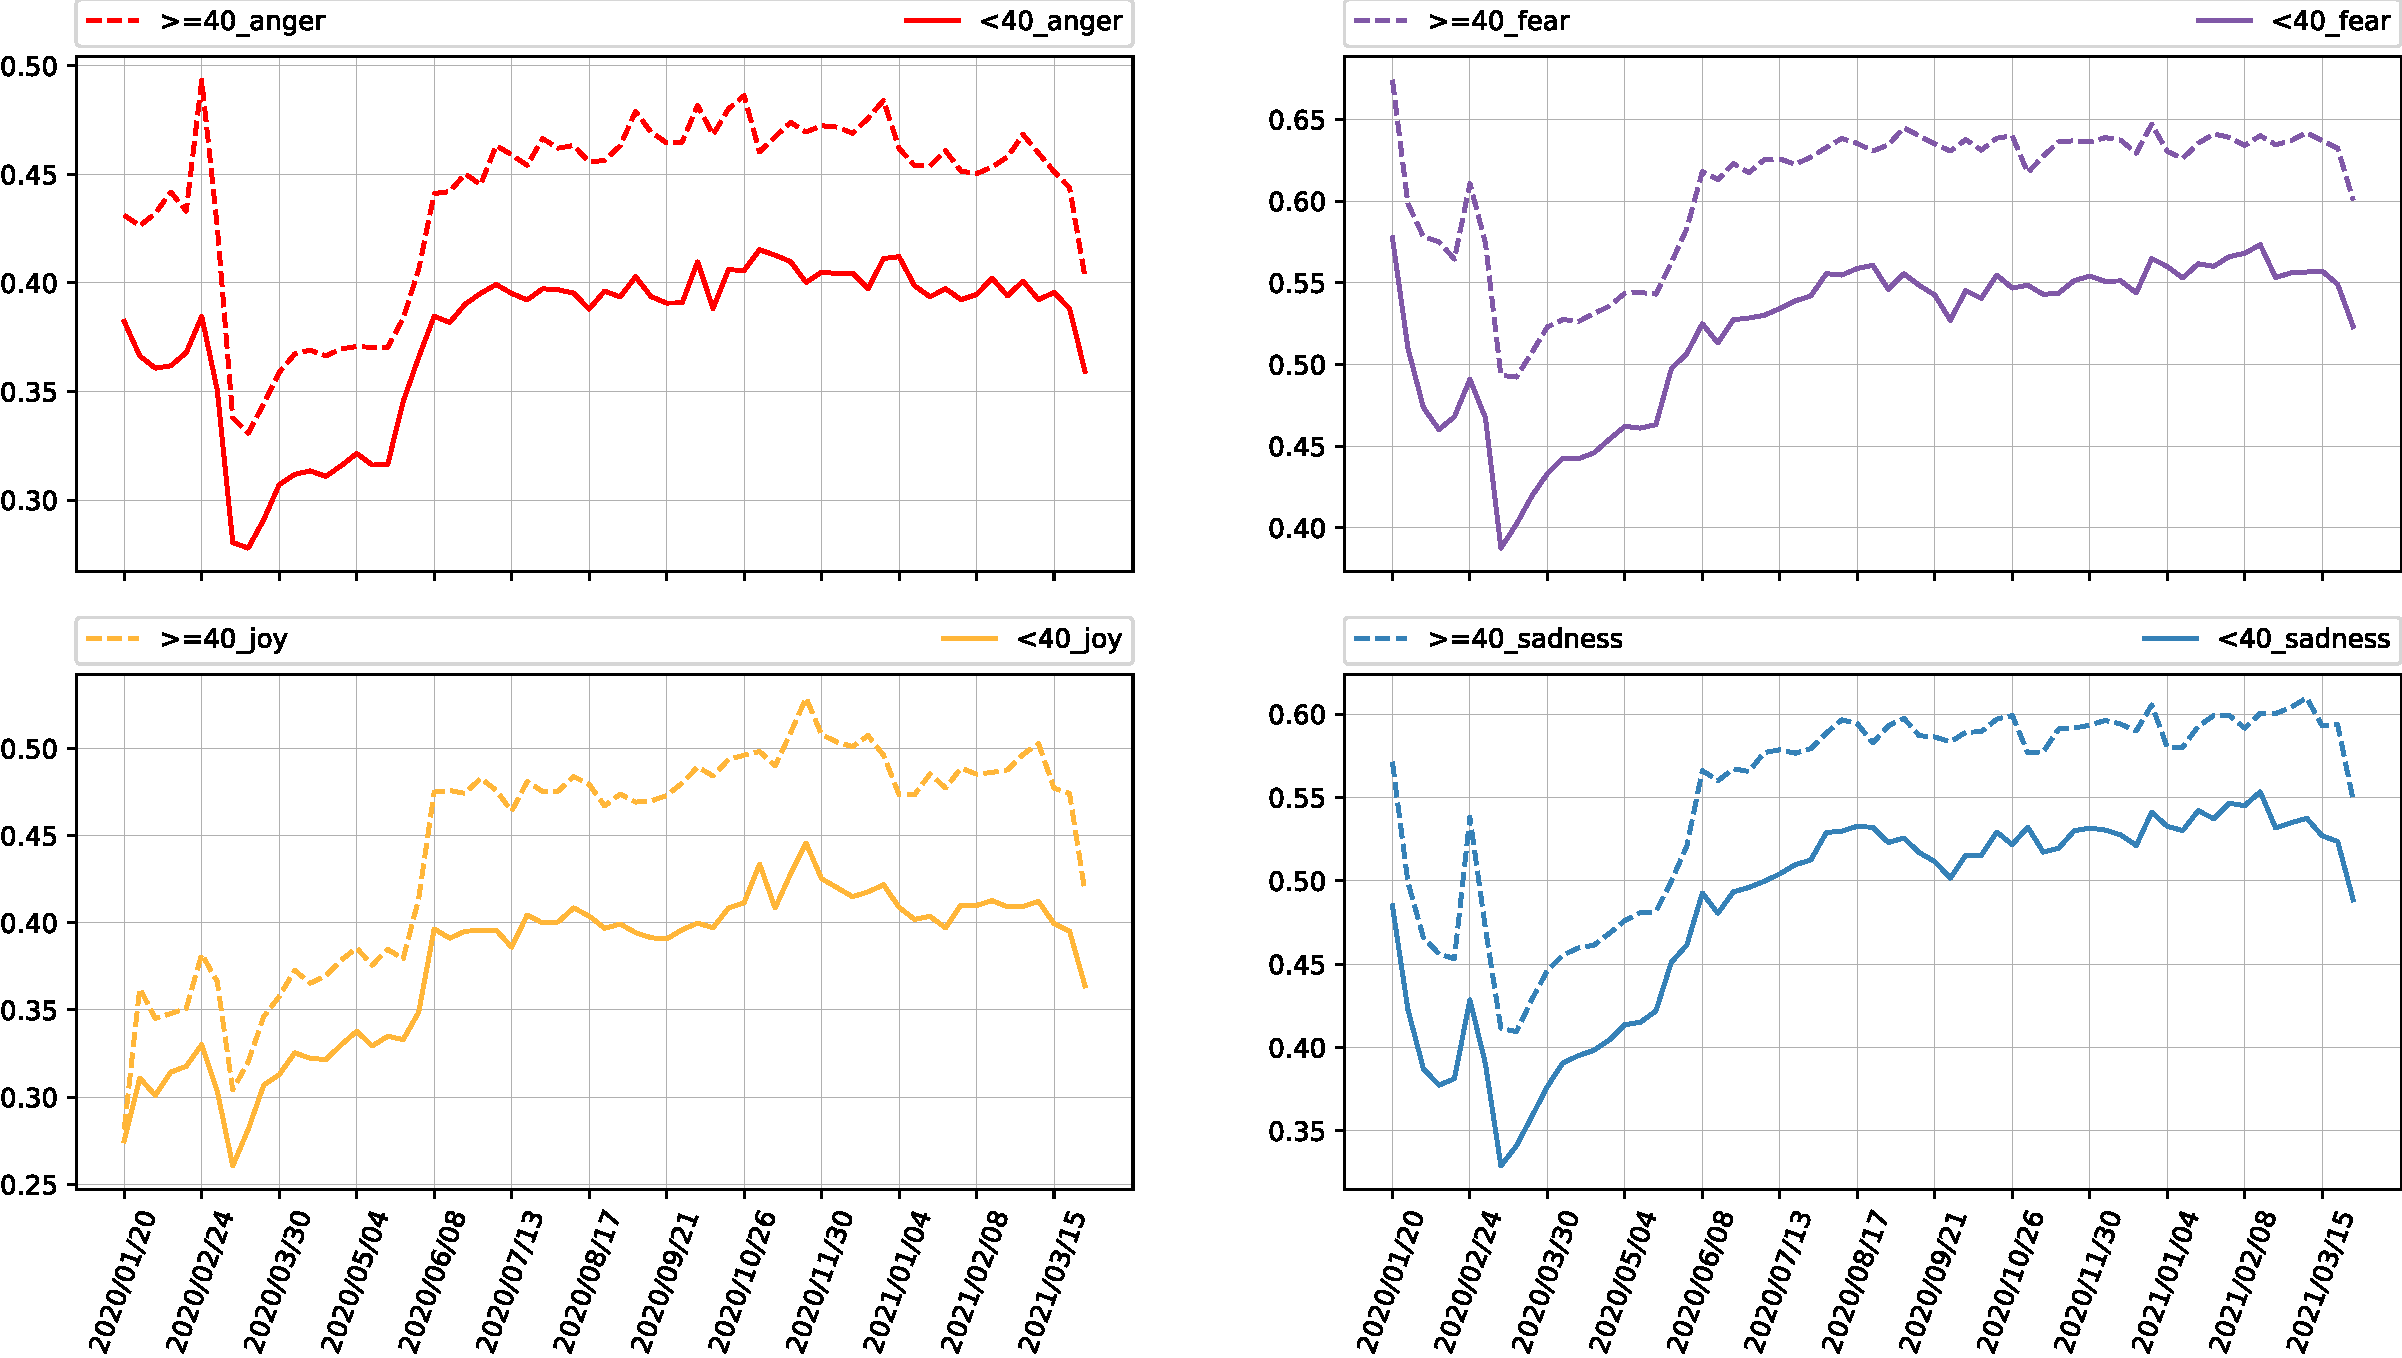
\includegraphics[scale=.25]{assets/img/en_4_emotions_per_age_subplot_1.svg.pdf}
    	\caption{Proportion of weekly users per age expressing a particular emotion in the English tweets}
    	\label{fig:en-4-emotions-per-age-subplot-1}
    \end{figure}
    
\end{frame}

\begin{frame}{Emotions expressed per state in the English tweets}

    \begin{figure}[H]
	    \centering
    	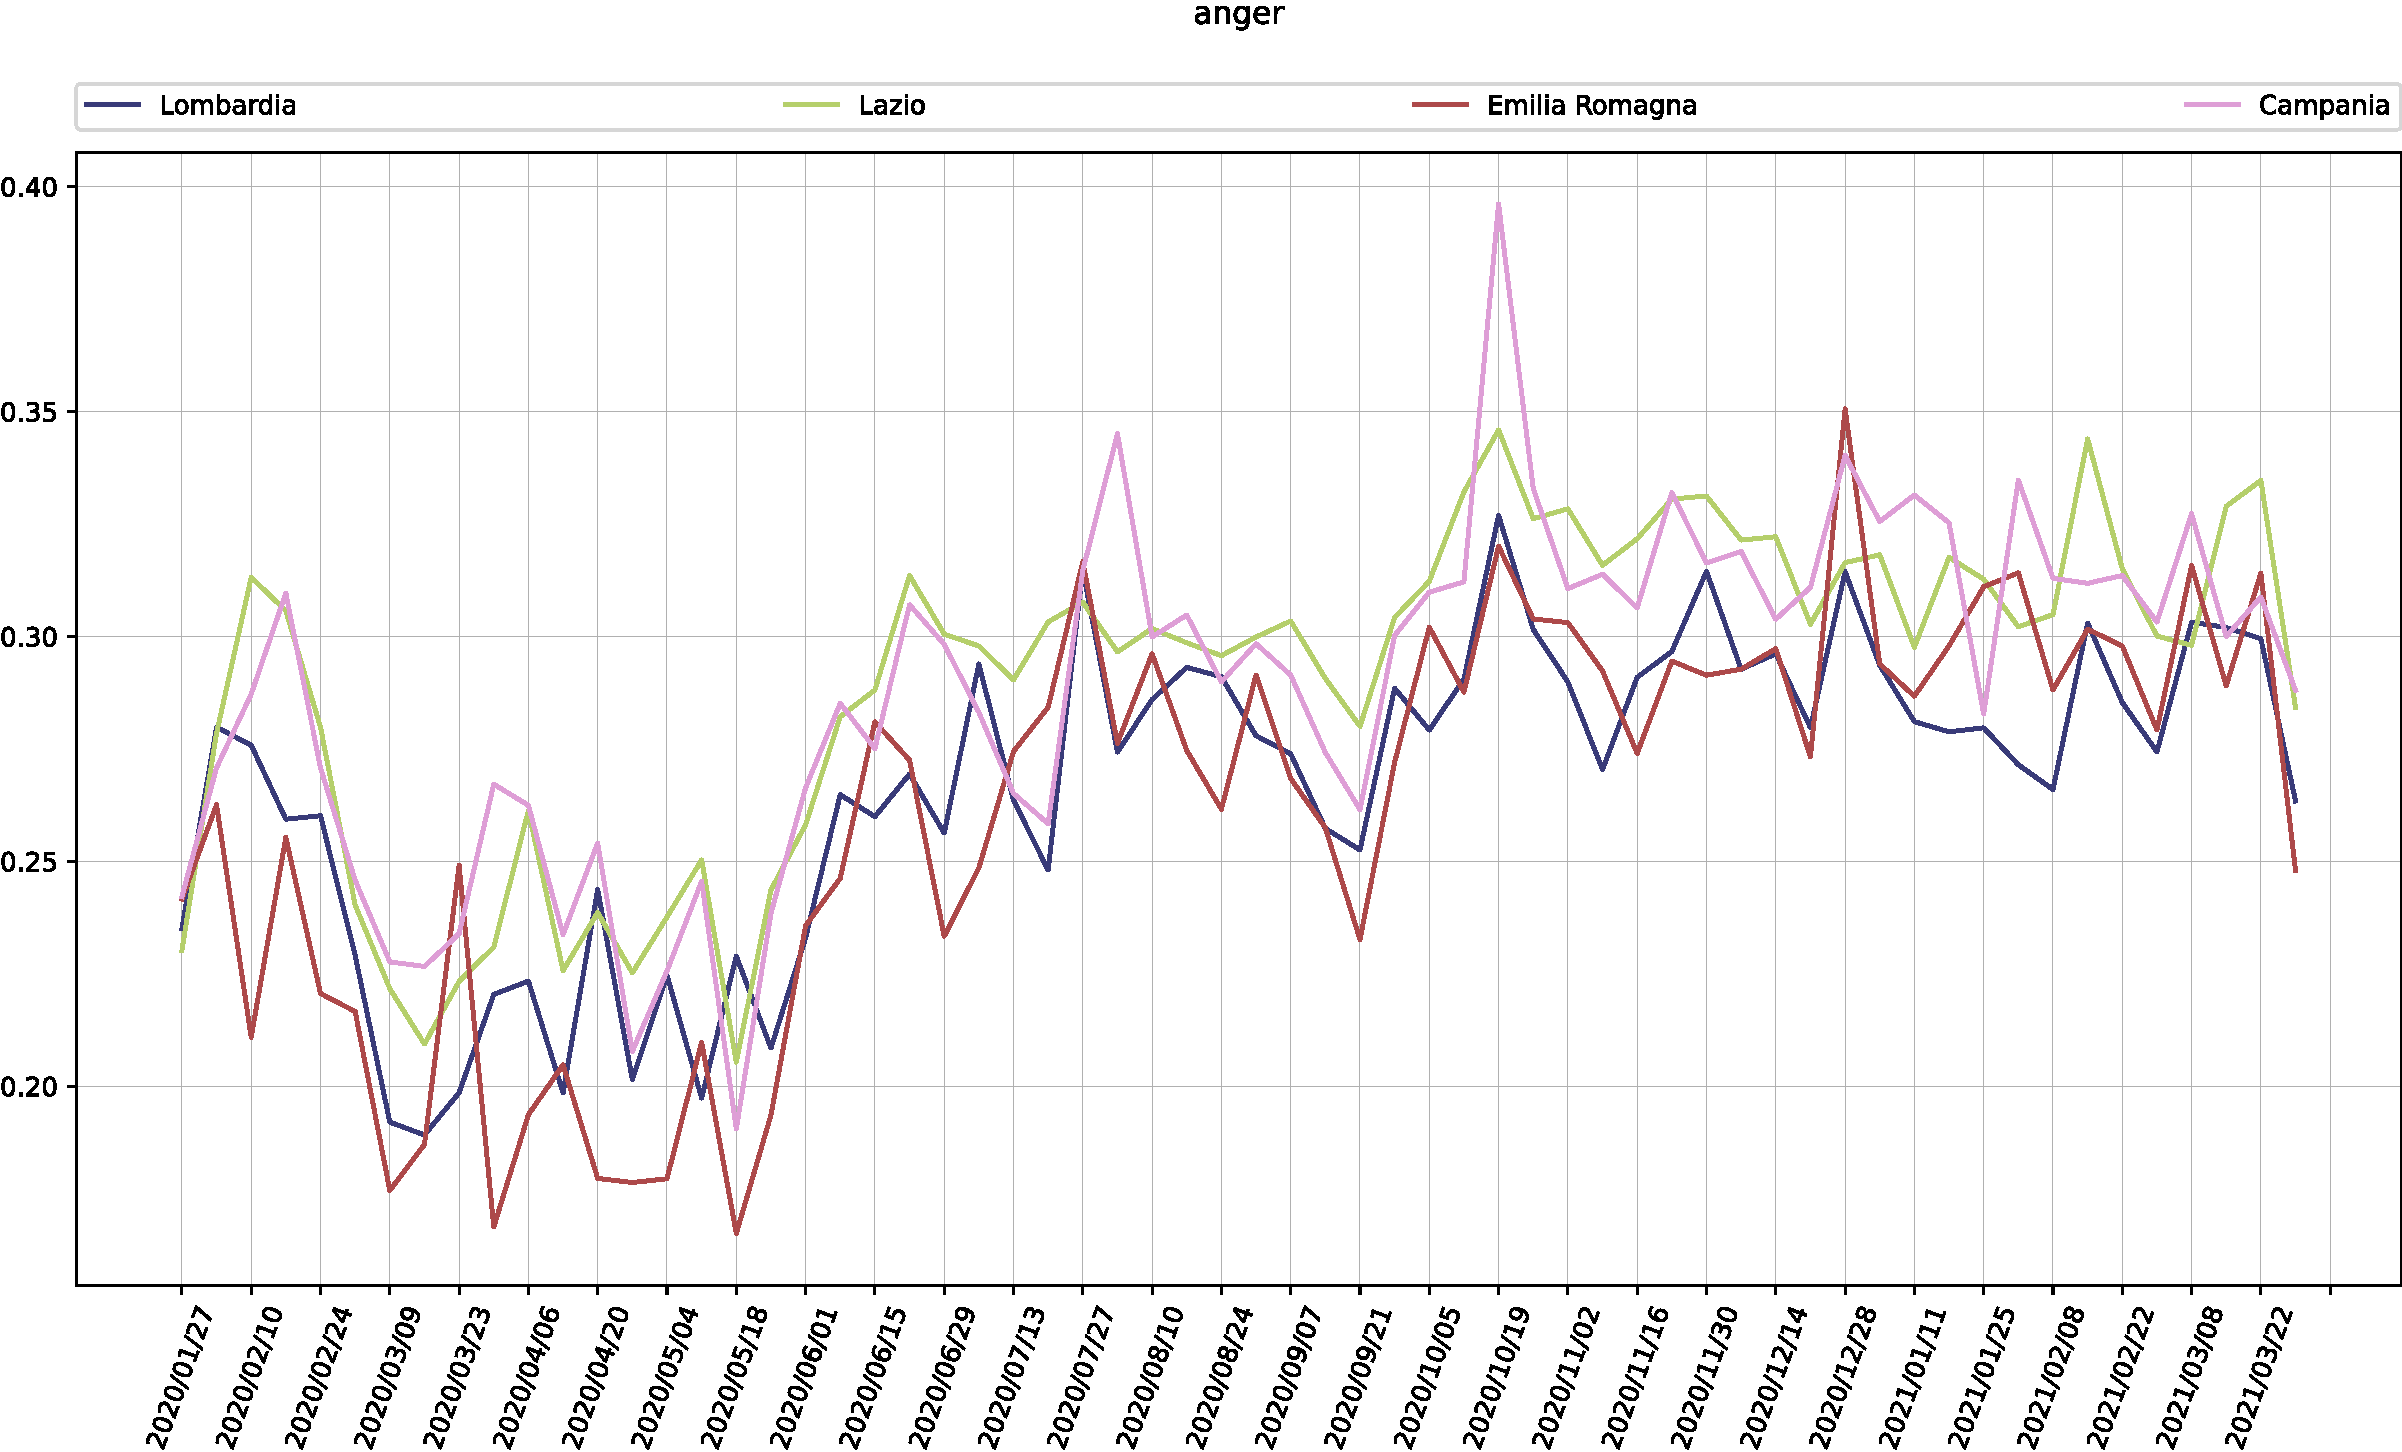
\includegraphics[scale=.25]{assets/img/it_anger_4_states.svg.pdf}
    	\caption{Proportion of weekly users that expressed anger in Lombardia, Lazio, Emilia Romagna and Campania}
    	\label{fig:it-anger-4-states}
    \end{figure}
    
\end{frame}

\section{Conclusions}

\begin{frame}{Next steps}
    
    Unfortunately, I was only able to scratch the surface of this research field. To improve some of the results, it would be possible to
    
    \begin{itemize}
        \item take into account the context of the words in a sentence using NLP algorithms to avoid opposite emotions bias
        \item use LIWC for more than validation
        \item build a dataset to link the emotional peaks to real events
    \end{itemize}
    
\end{frame}

\begin{frame}

    \begin{center}
        \Large{Thanks for the attention.}
    \end{center}

\end{frame}

\begin{frame}[allowframebreaks,plain,noframenumbering]
        \frametitle{References}
        \printbibliography
\end{frame}






%% Additional Slides for questions






\begin{frame}[plain,noframenumbering]{Tools and Libraries used}

    \begin{itemize}
        \item Python, as main programming language to write the code for the project
        \item Pandas, to perform small operation on the datasets
        \item Matplotlib and Plotly, for data visualization
        \item Twarc, to retrieve (hydrate) tweets from Twitter using TweetIDs
        \item m3inference, a deep learning system for demographic inference (gender, age, and person/organization)
        \item geopy and Nominatim, to geocode the locations of the users
        \item NRC Word-Emotion Association Lexicon (aka EmoLex), to perform sentiment analysis on the tweets of the users
    \end{itemize}
    
\end{frame}

\begin{frame}[plain,noframenumbering]{Languages with the most tweets}
    
    \begin{table}[H]
        \centering
        \ra{1.2}
        \begin{tabularx}{\columnwidth}{@{}llrrrr@{}}
        		\bottomrule
        		\textbf{language} & \textbf{ISO} & \textbf{unique tweets} & \textbf{retweets} & \textbf{total} & \textbf{percentage} \\
        		\midrule
            English & en & 195 645 826 & 473 950 322 & 669 596 148 & 63.41\% 
            \\
    		Spanish & es & 35 533 886 & 111 464 189 & 146 998 075 & 13.92\% 
    		\\
    		Portuguese & pt & 15 459 760 & 29 912 427 & 45 372 187 & 4.30\% 
    		\\
    		French & fr & 9 547 251 & 23 635 273 & 33 182 524 & 3.14\% 
    		\\
    		Indonesian & in & 9 029 012 & 16 479 537 & 25 508 549 & 2.41\%
    		\\
    		German & de & 8 091 516 & 11 447 554 & 19 539 070 & 1.85\%
    		\\
    		Japanese & ja & 3 228 542 & 10 220 609 & 13 449 151 & 1.27\%
    		\\
    		Italian & it & 5 256 748 & 7 173 234 & 12 429 982 & 1.18\%
    		\\
    		Turkish & tr & 3 347 597 & 6 698 252 & 10 045 849 & 0.95\%
    		\\
    		Thai & th & 350 268 & 9 028 730 & 9 378 998 & 0.89\%
    		\\
    		\bottomrule
        \end{tabularx}
        \caption{Top 10 languages with the most tweets}
        \label{tab:dataset-language-stats}
    \end{table}

\end{frame}

\begin{frame}[plain,noframenumbering]{Tweets over time}

    \begin{figure}[H]
    	\centering
    	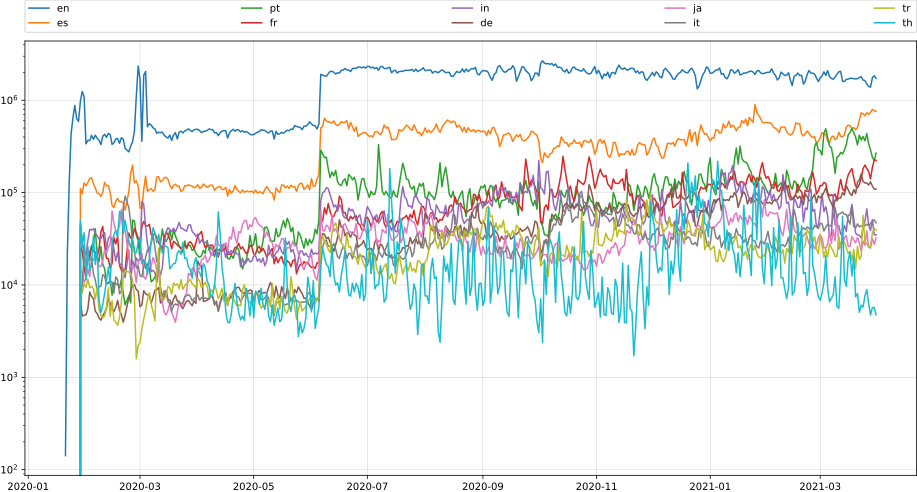
\includegraphics[scale=.25]{assets/img/tweets_per_language_over_time}
    	\caption{Number of tweets in logarithmic scale over time for the top 10 languages}
    	\label{fig:tweets-language-over-time}
    \end{figure}

\end{frame}

\begin{frame}[plain,noframenumbering]{Data organization}

	To access directly to a specific category of tweets (e.g. the tweets written in English on the 3rd of June 2020), we grouped them 
	
	\begin{itemize}
	    \item first according to the \textbf{language}, using the \texttt{lang} field from Twitter
	    \item secondly by \textbf{year-month}
	    \item and finally by \textbf{day}
	\end{itemize}
	
    Later on, we decided to \textbf{aggregate them in weekly batches} for a clearer visualization and to average the results.

\end{frame}

\begin{frame}[plain,noframenumbering]{Personal contribution to m3inference}

	During the project I encountered several errors while using m3inference, for this reason I decided to open a Pull Request on GitHub\footnote{Pull request: \href{https://github.com/euagendas/m3inference/pull/20}{fix urllib errors while trying to fetch a profile image from twitter \#20}} to contribute to the project.
	
	\begin{figure}
	    \centering
	    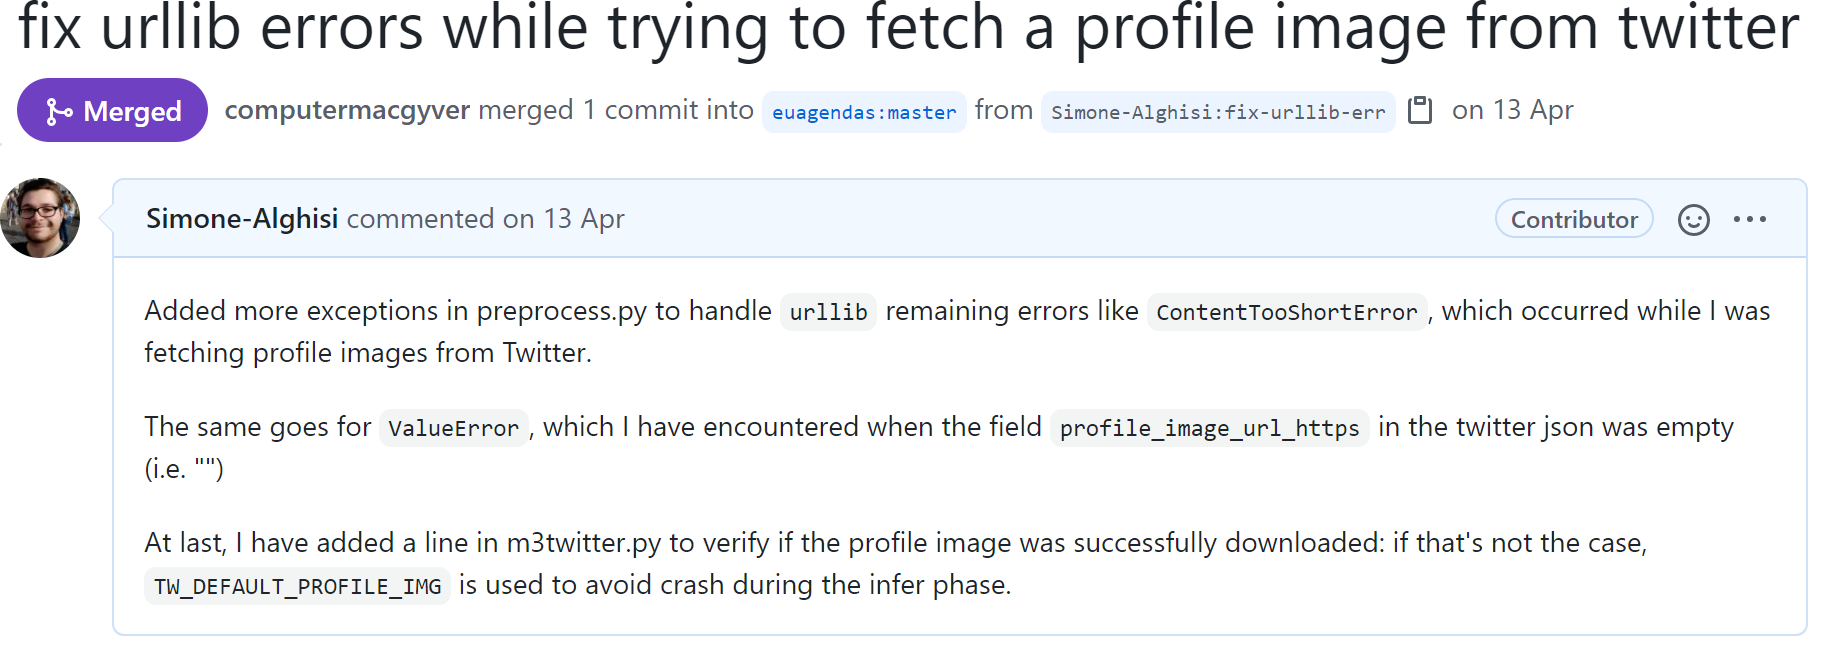
\includegraphics[scale=0.165]{assets/img/pull_request.png}
	\end{figure}
	
	The version of m3inference on the packet manager was updated when the same issue was notified by another user\footnote{issue: \href{https://github.com/euagendas/m3inference/issues/21}{Error fetching images will fail the infer method \#21}}.
	
\end{frame}

\begin{frame}[plain,noframenumbering]{Valid users - gender}

    \begin{definition}
    \label{def:valid-users}
    	A user \(u\) belongs to the category \(c \in C\) iif their prediction confidence \(pc\) is greater or equal than 0.95, i.e.
    	\[u \in c \Longleftrightarrow pc(u, c) \geq 0.95\]
    \end{definition}
    	
    In particular, the following methodology was applied:
    	
    \begin{itemize}
    	\item first we check if the user's account belongs to an organization
    	\item then, if the user is male (or female)
    	\item finally, if none of the previous constraints were satisfied, we do not consider this user
    \end{itemize}
    
\end{frame}

\begin{frame}[plain,noframenumbering]{Valid users - age}

    \begin{definition}
    \label{def:valid-users-age}
    	A user \(u\) belongs to the age bracket \(a \in A\) iif their prediction confidence \(pc\) is greater or equal than 0.95, i.e.
    	\[u \in a \Longleftrightarrow pc(u, a) \geq 0.95\]
    \end{definition}
    
    To consider only the users that comply with \Cref{def:valid-users-age}, we applied the following methodology:
    
    \begin{itemize}
    	\item first we check if \(pc(u, \texttt{>=40}) \geq 0.95\)
    	\item then, if \(1 - pc(u, \texttt{>=40}) \geq 0.95\) (i.e. if they have less than forty years)
    	\item finally, if none of the previous constraints were satisfied, we do not consider this user
    \end{itemize}
    
\end{frame}

\begin{frame}[plain,noframenumbering]{Valid users - statistics}

    \begin{table}[h]
    	\centering
    	\ra{1.2}
    	\begin{tabular}{lrrrrrr}
    		\toprule
    		\textbf{language} & \textbf{inferred users} & \textbf{valid users} & \textbf{males \%} & \textbf{females \%} & \textbf{orgs \%}
    		\\
    		\midrule
    		Catalan & 98 132 & 73 835 & 67.30 & 22.95 & 9.75
    		\\
    		English & 3 099 883 & 2 335 112 & 63.88 & 32.16 & 3.96 
    		\\
    		Italian & 217 340 & 167 093 & 67.21 & 27.96 & 4.83 
    		\\
    		Spanish & 2 555 941 & 2 029 765 & 63.88 & 33.23 & 2.89 
    		\\
    		\bottomrule
    	\end{tabular}
    	\caption{General users statistics for Catalan, English, Italian and Spanish tweets (gender)}
    	\label{tab:users-languages}
    \end{table}
    
    \begin{table}[h]
    	\centering
    	\ra{1.2}
    	\begin{tabular}{lrrrr}
    		\toprule
    		\textbf{language} & \textbf{inferred users} & \textbf{valid users} & \(< \textbf{40 \%}\) & \(\geq \textbf{40 \%}\) 
    		\\
    		\midrule
    		Catalan & 98 132 & 42 383 & 57.83 & 42.17
    		\\
    		English & 3 099 883 & 1 717 733 & 68.84 & 33.16 
    		\\
    		Italian & 217 340 & 122 271 & 64.54 & 35.46 
    		\\
    		Spanish & 2 555 941 & 1 542 935 & 84.82 & 15.18
    		\\
    		\bottomrule
    	\end{tabular}
    	\caption{General users statistics for Catalan, English, Italian and Spanish tweets (age)}
    	\label{tab:users-age}
    \end{table}
    
\end{frame}

\begin{frame}[plain,noframenumbering]{Data normalization (categories)}
	
	We also wanted to study whether a certain category \(c \in C\) expressed at time \(t\) more (or less) emotion \(e\) (e.g. sadness, anger) w.r.t the mean value for emotion \(e\) in the period of time \([0, T]\), regardless of the category.

    For this reason, we applied \Cref{def:categories-normalization} to our data:
    	
    \begin{definition}
    \label{def:categories-normalization}
    	Given \(f_{e, c}(t)\), i.e. the proportion of users belonging to category \(c \in C\) that expressed emotion \(e\) at time \(t\), and the period of time \([0,T]\),
    	
    	\[v_{e, c}(t) = \frac{f_{e, c}(t) - \mu_{[0,T]}(f_e)}{\mu_{[0,T]}(f_e)}\]
    	
    	\[\text{where } \mu_{[0,T]}(f_e) = \frac{1}{\mid T \mid} \sum_{t =0}^{T} f_e(t) = \frac{1}{\mid T \mid} \sum_{t =0}^{T} \sum_{c \in C} f_{e, c}(t)\] 
    \end{definition}
	
\end{frame}

\begin{frame}[plain,noframenumbering]{Comparison between EmoLex and LIWC}

    \begin{figure}[H]
	    \centering
    	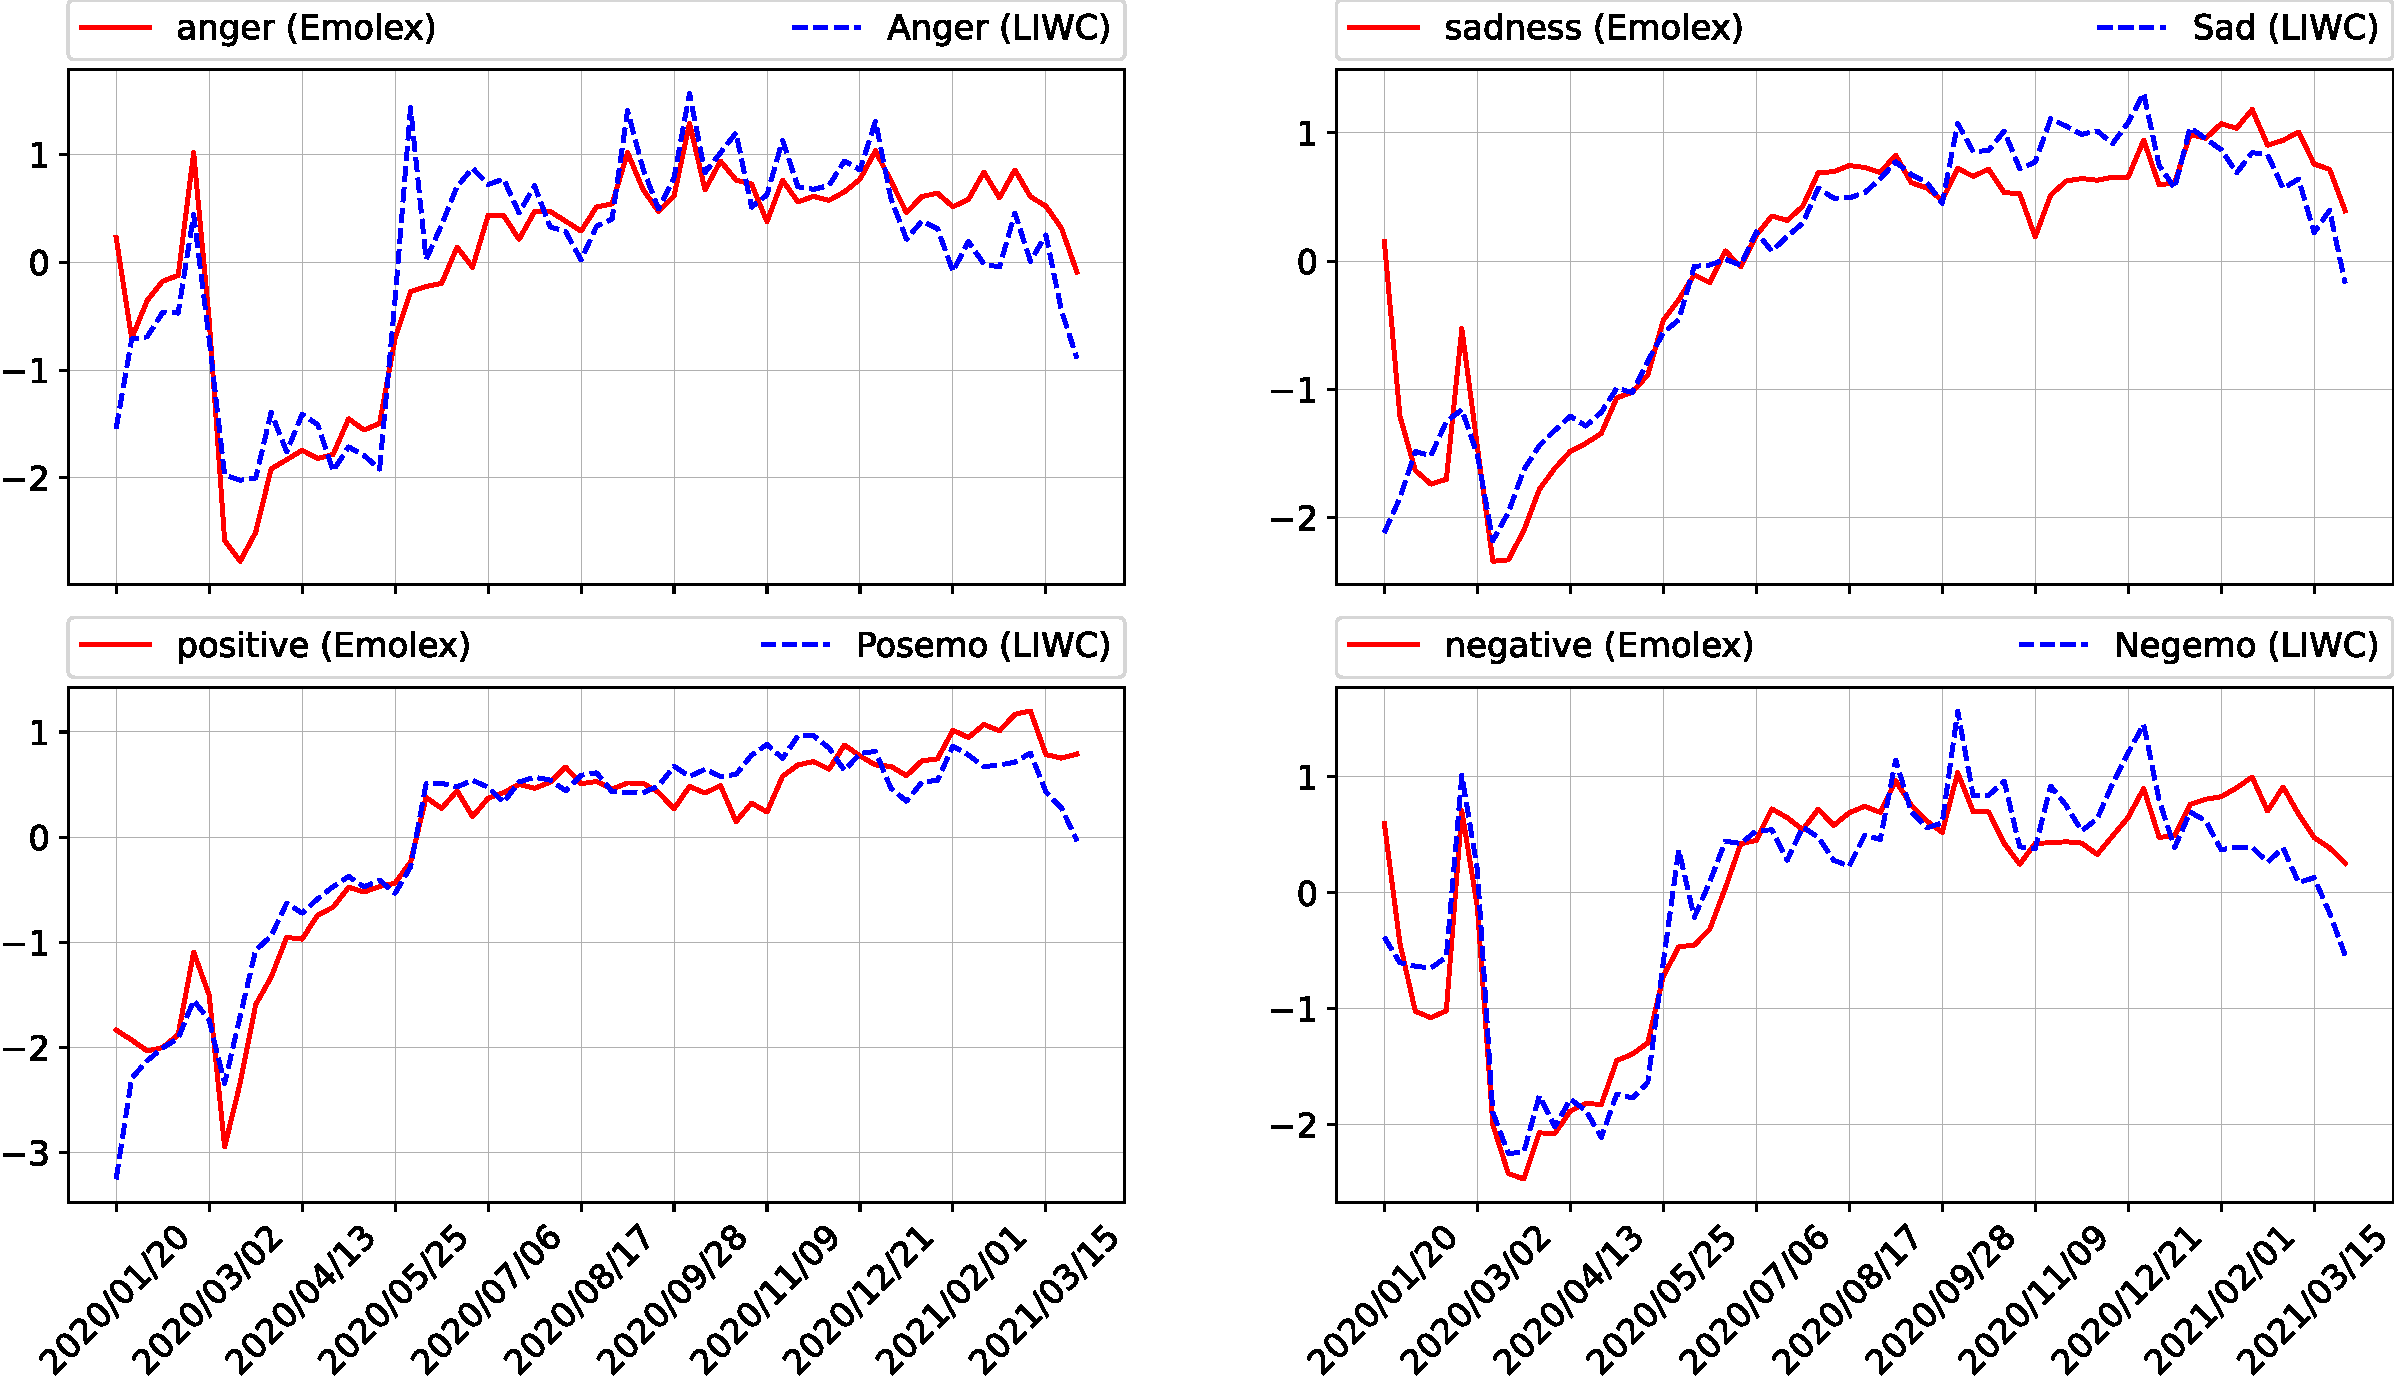
\includegraphics[scale=.25]{assets/img/en_emotions_and_liwc_categories_comparison.svg.pdf}
    	\caption{Comparison between the z-score of the emotions and the z-score of the LIWC categories}
    	\label{fig:en-emotions-liwc-comparison}
    \end{figure}
    
\end{frame}

\begin{frame}[plain,noframenumbering]{Emotion in the English tweets (subplots)}

    \begin{figure}[H]
	    \centering
    	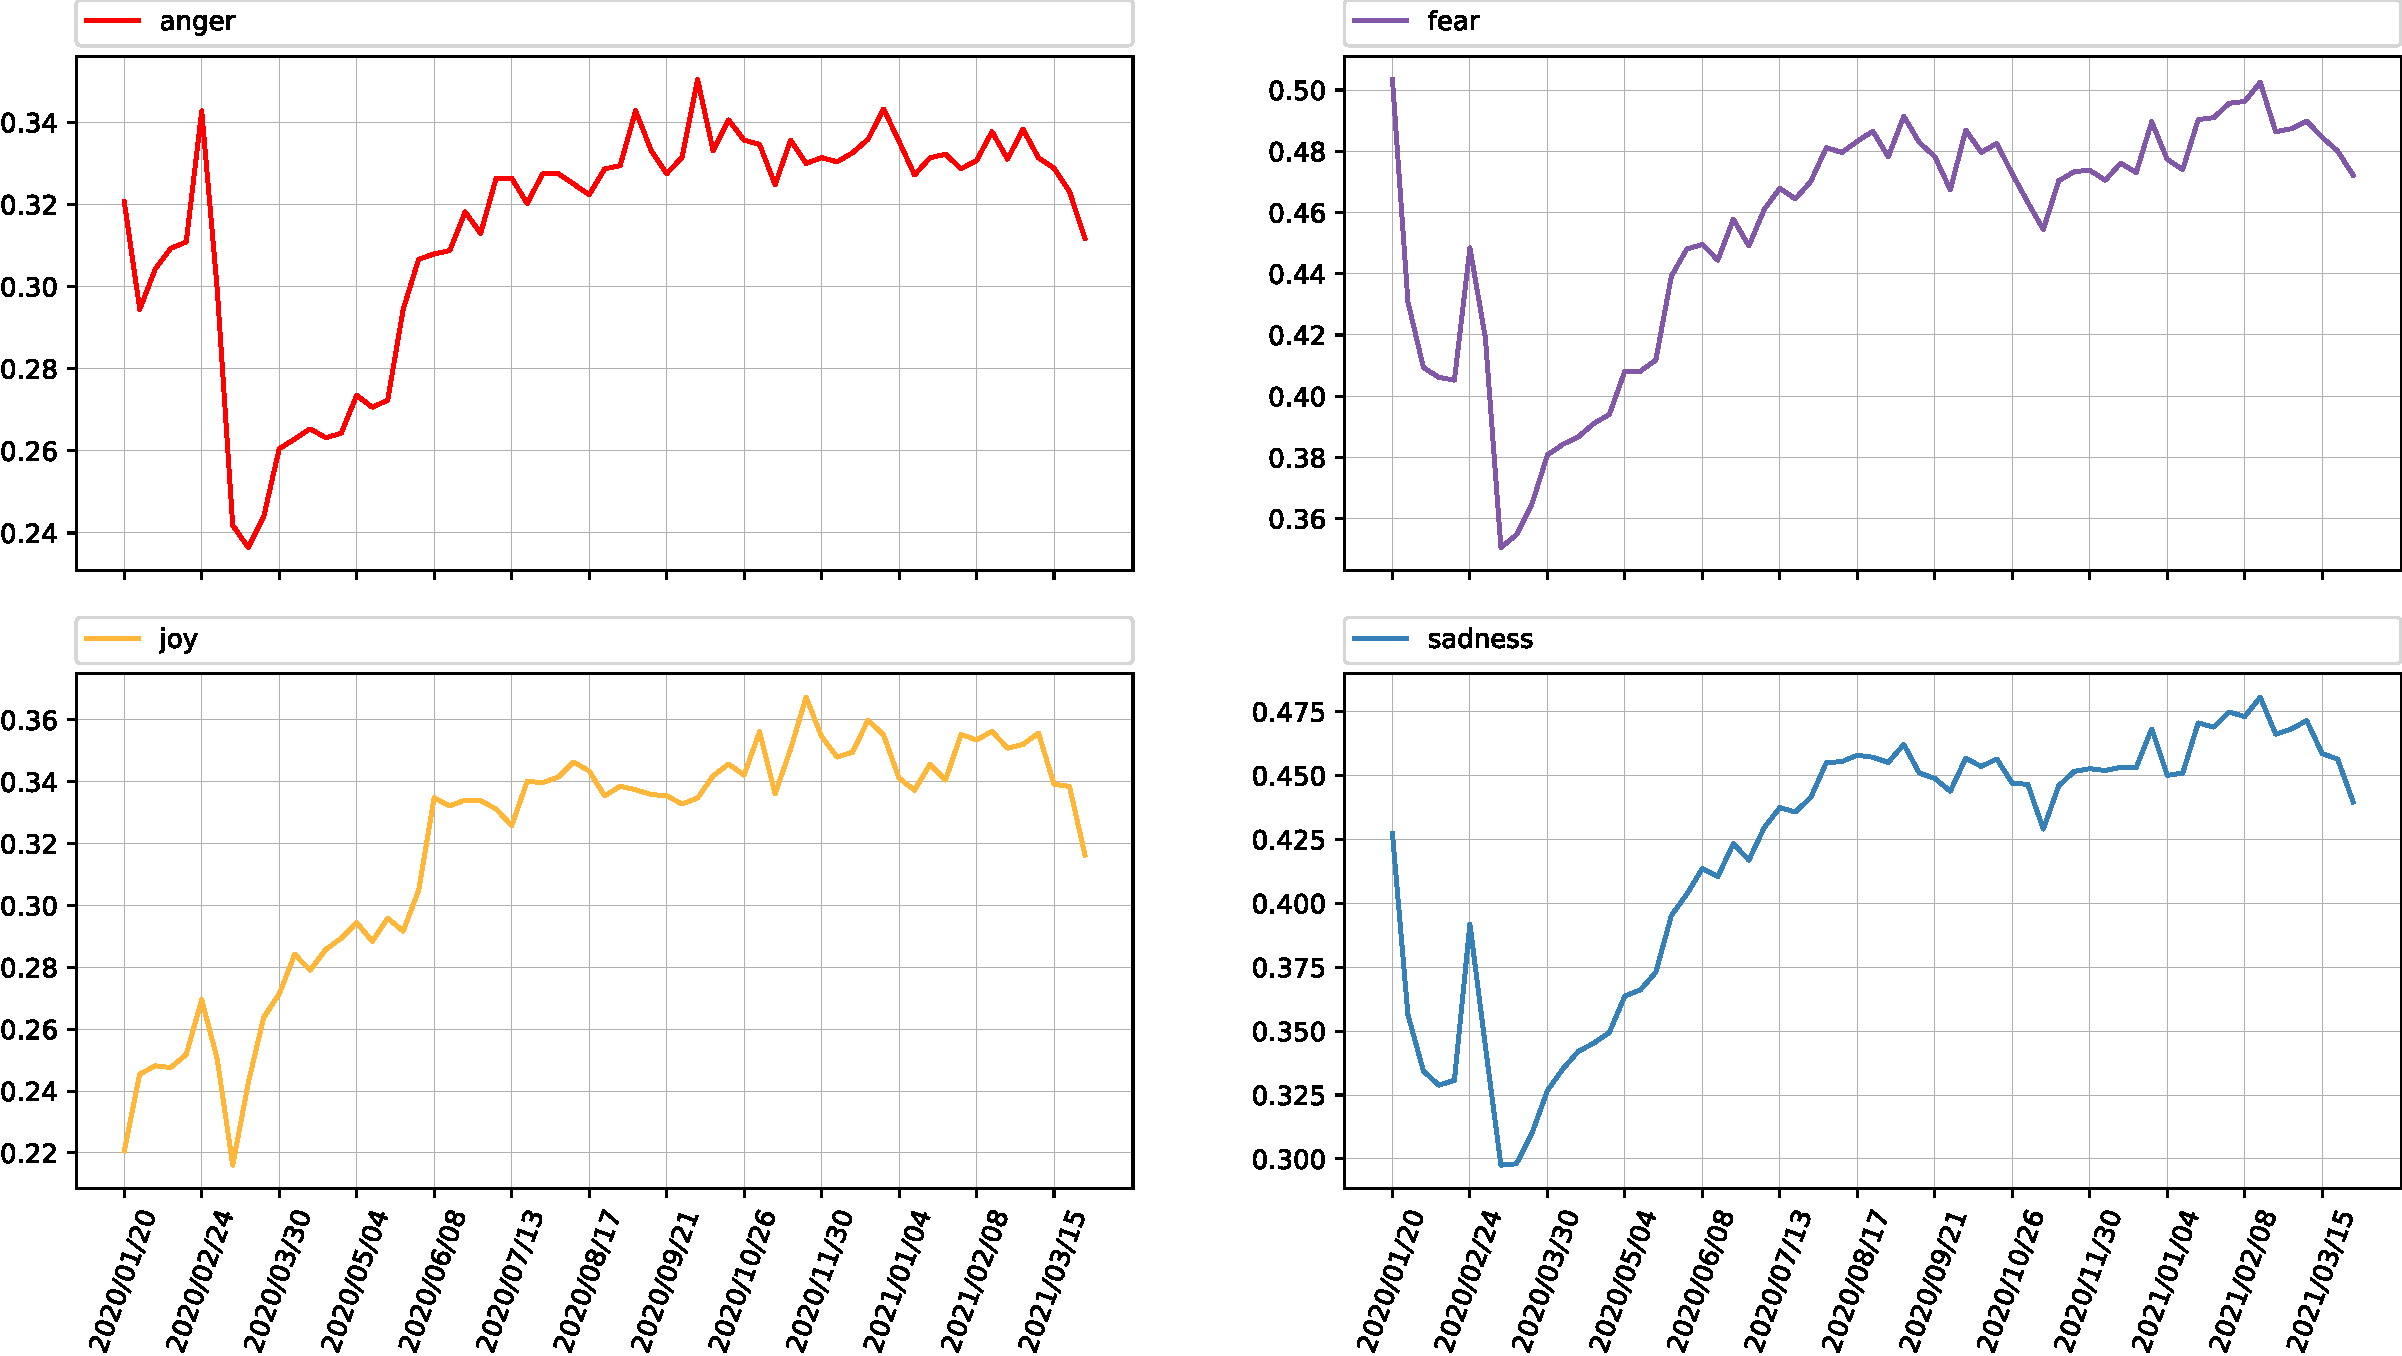
\includegraphics[scale=.25]{assets/img/en_4_emotions_subplot_1.svg.pdf}
    	\caption{Proportion of weekly users expressing a particular emotion in the English tweets}
    	\label{fig:en-4-emotions-subplot-1}
    \end{figure}
    
\end{frame}

\begin{frame}[plain,noframenumbering]{Most used words on 2020/02/24 in the English tweets}

    \begin{figure}[H]
	    \centering
    	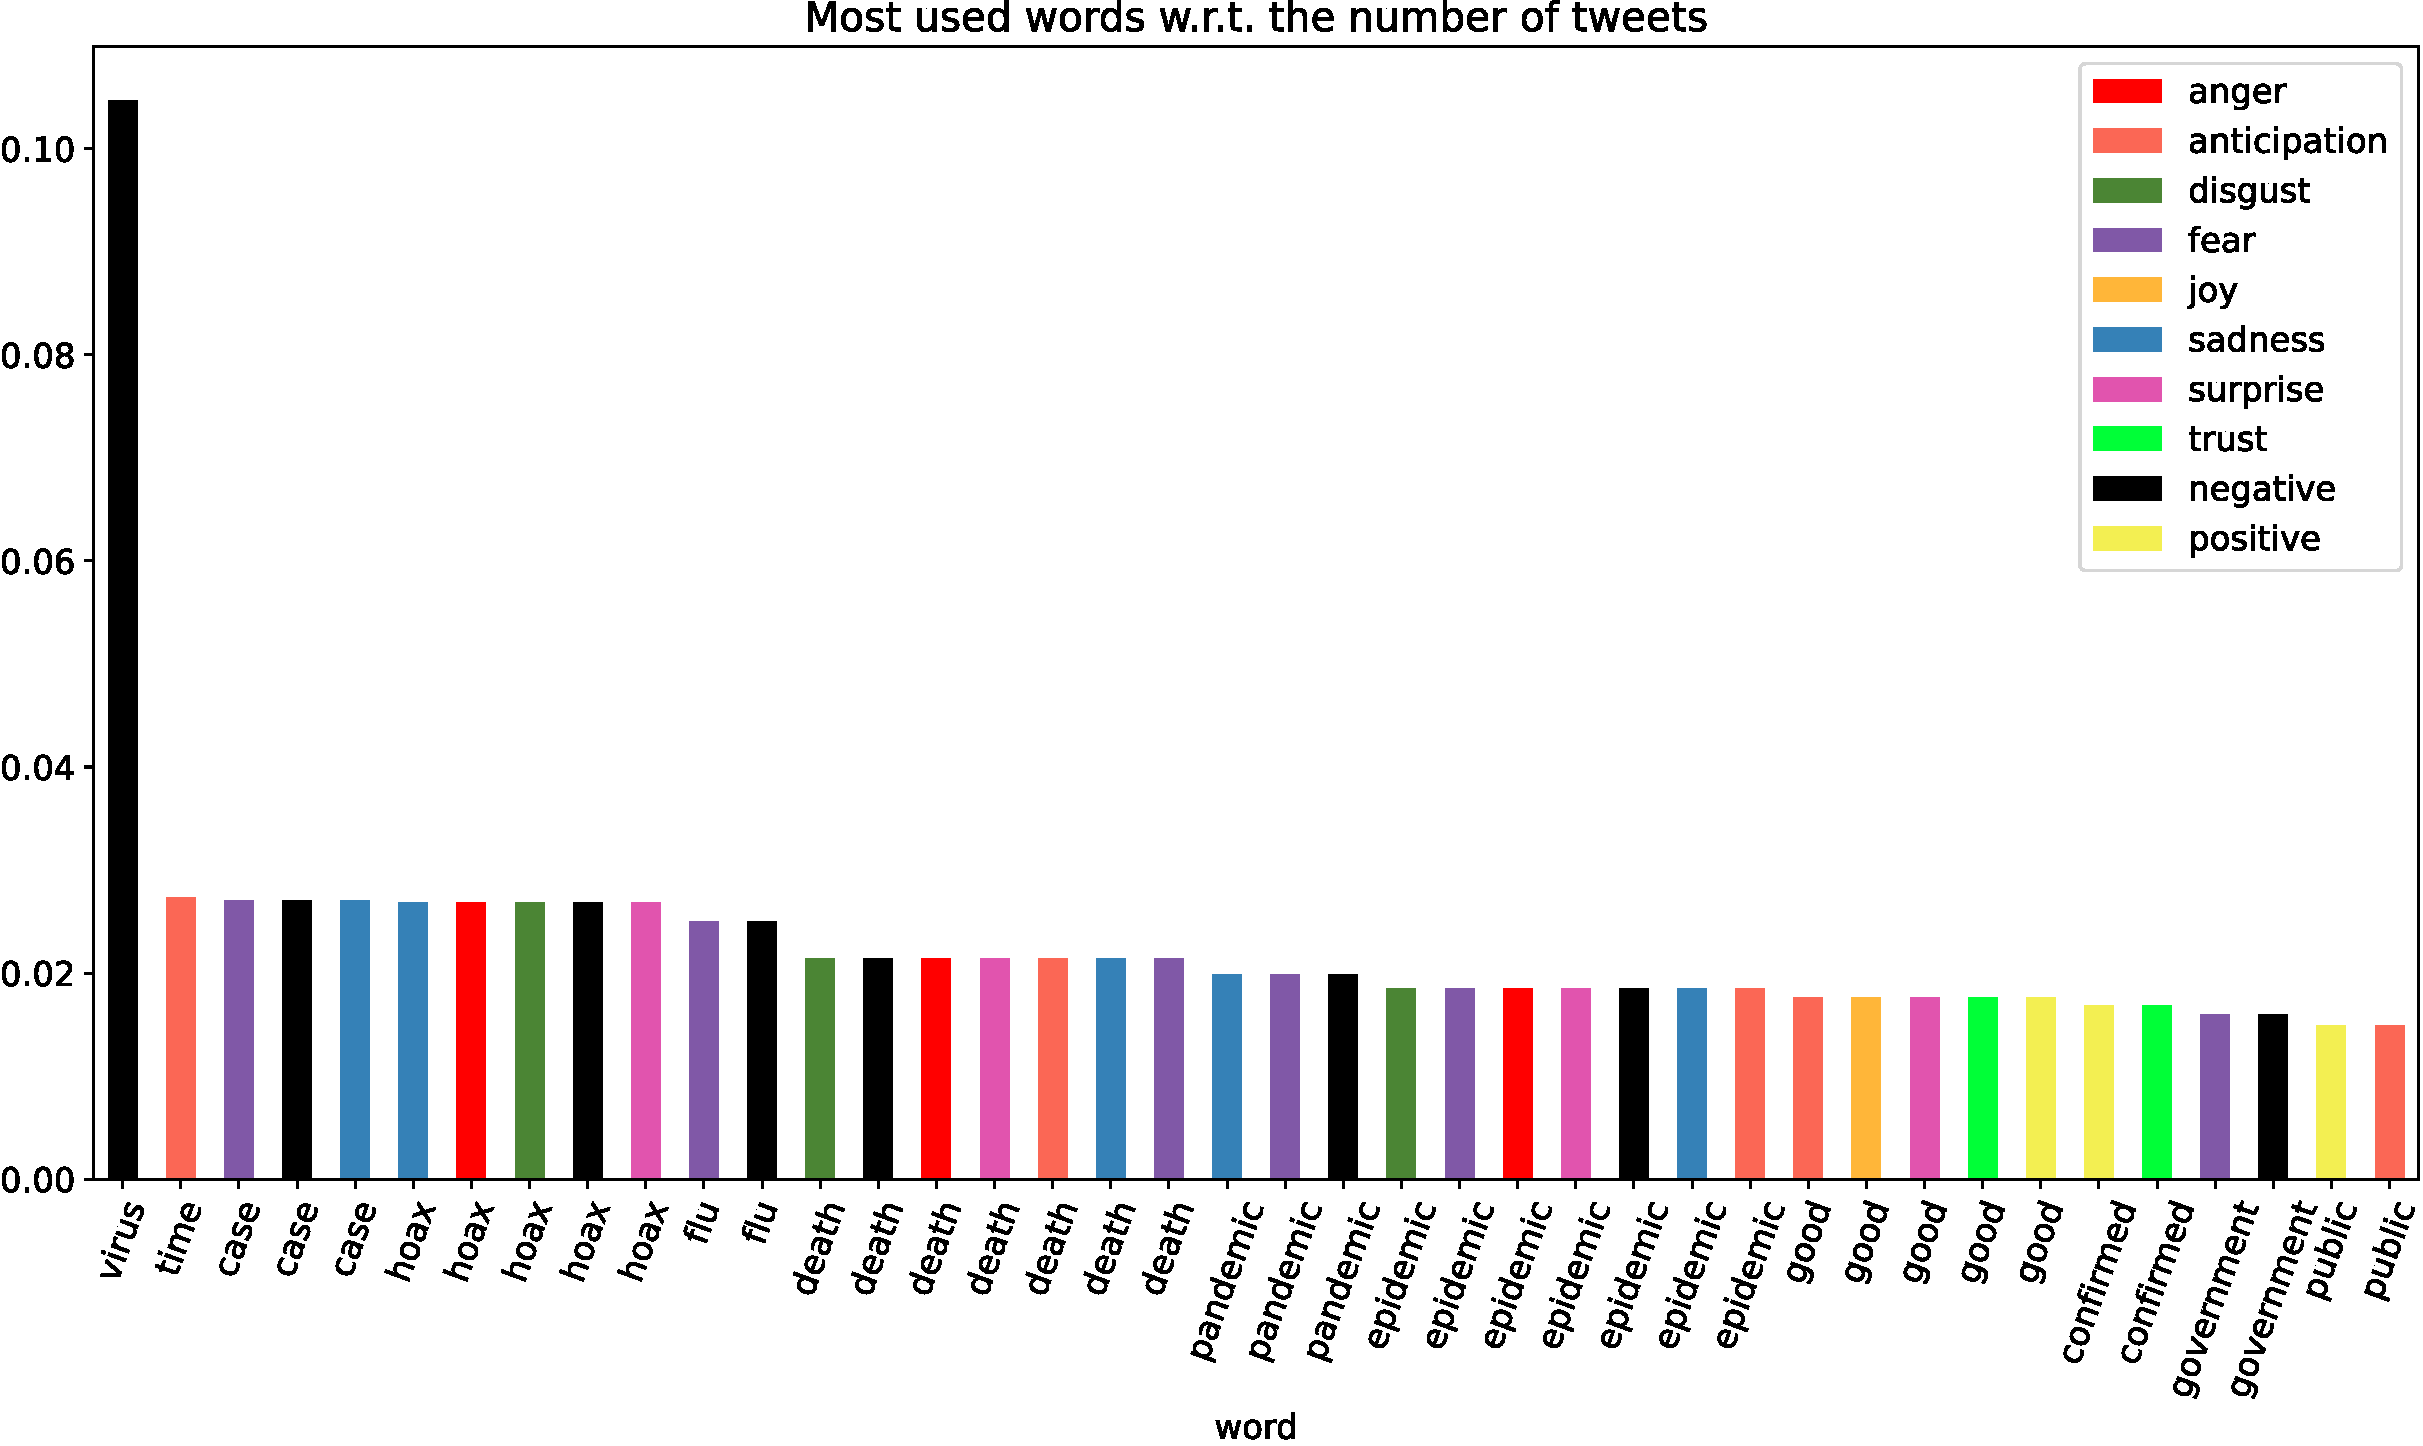
\includegraphics[scale=.25]{assets/img/en_most_used_words_2020_02_24.svg.pdf}
    	\caption{Proportion of most used words on 2020/02/24 that express emotion/sentiment in the English tweets}
    	\label{fig:en-most-used-word-2020-02-24}
    \end{figure}
    
\end{frame}

\begin{frame}[plain,noframenumbering]{Most used words per emotions on 2020/02/24 in the English tweets}

    \begin{figure}[H]
	    \centering
    	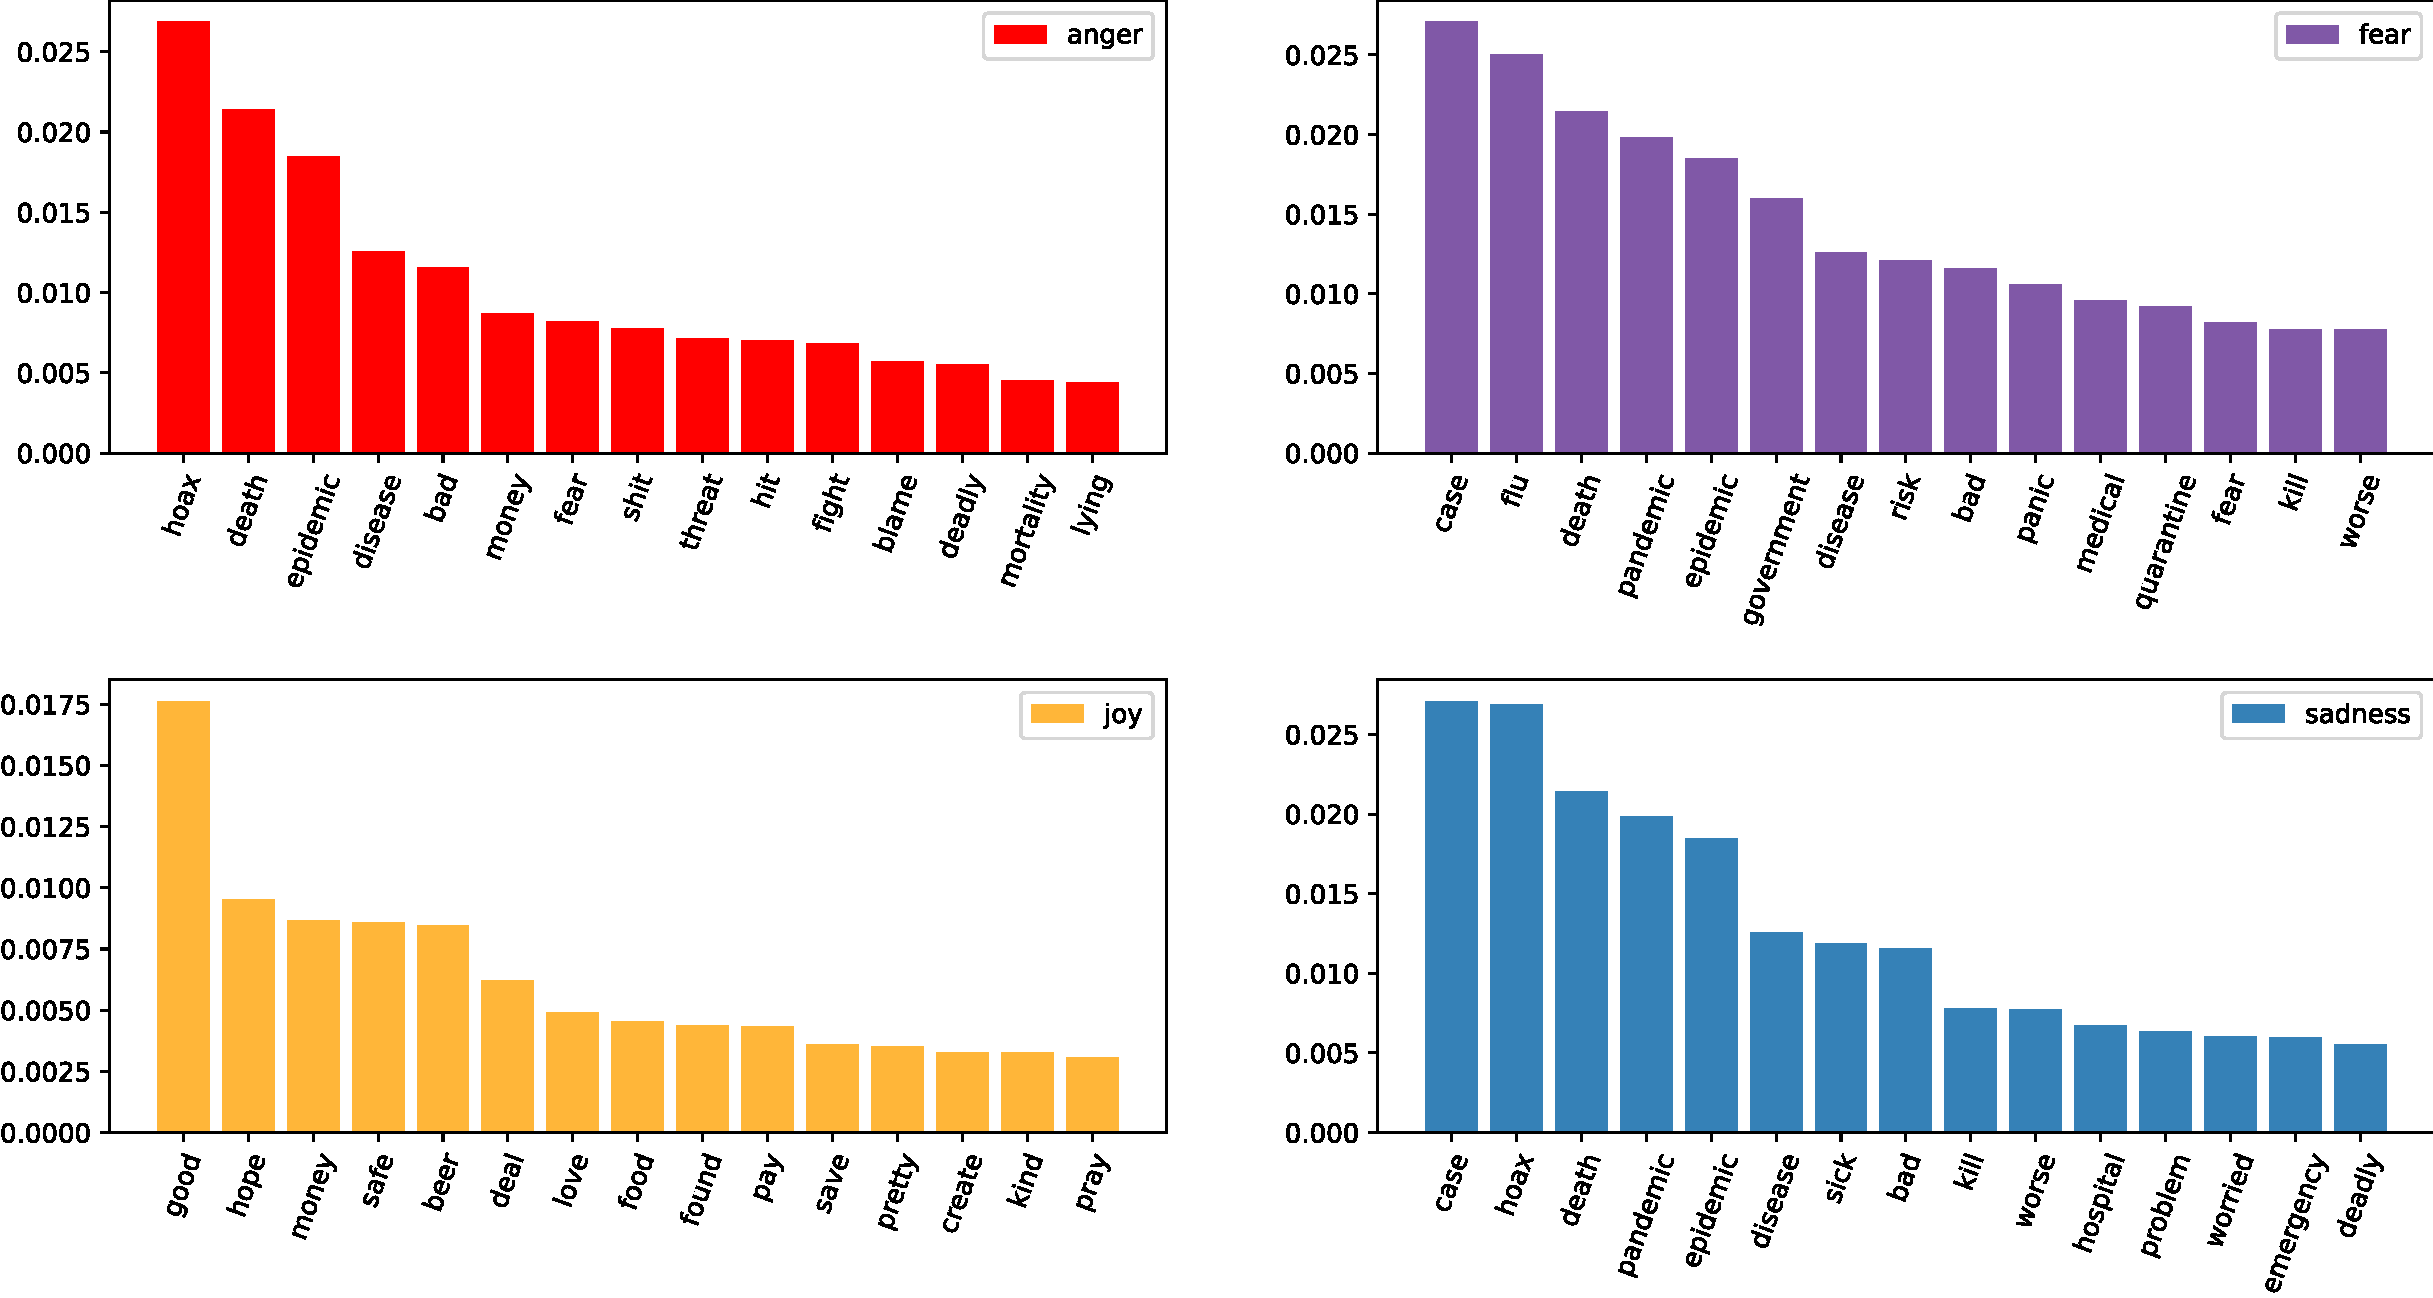
\includegraphics[scale=.25]{assets/img/en_most_used_words_4_emotions_2020_02_24_subplot.svg.pdf}
    	\caption{Proportion of 15 most used words on 2020/02/24 per emotion in the English tweets}
    	\label{fig:en-most-used-word-subplot-2020-02-24}
    \end{figure}
    
\end{frame}

\begin{frame}[plain,noframenumbering]{Number of emotions per age for a given week in the English tweets}

    \begin{figure}[H]
	    \centering
    	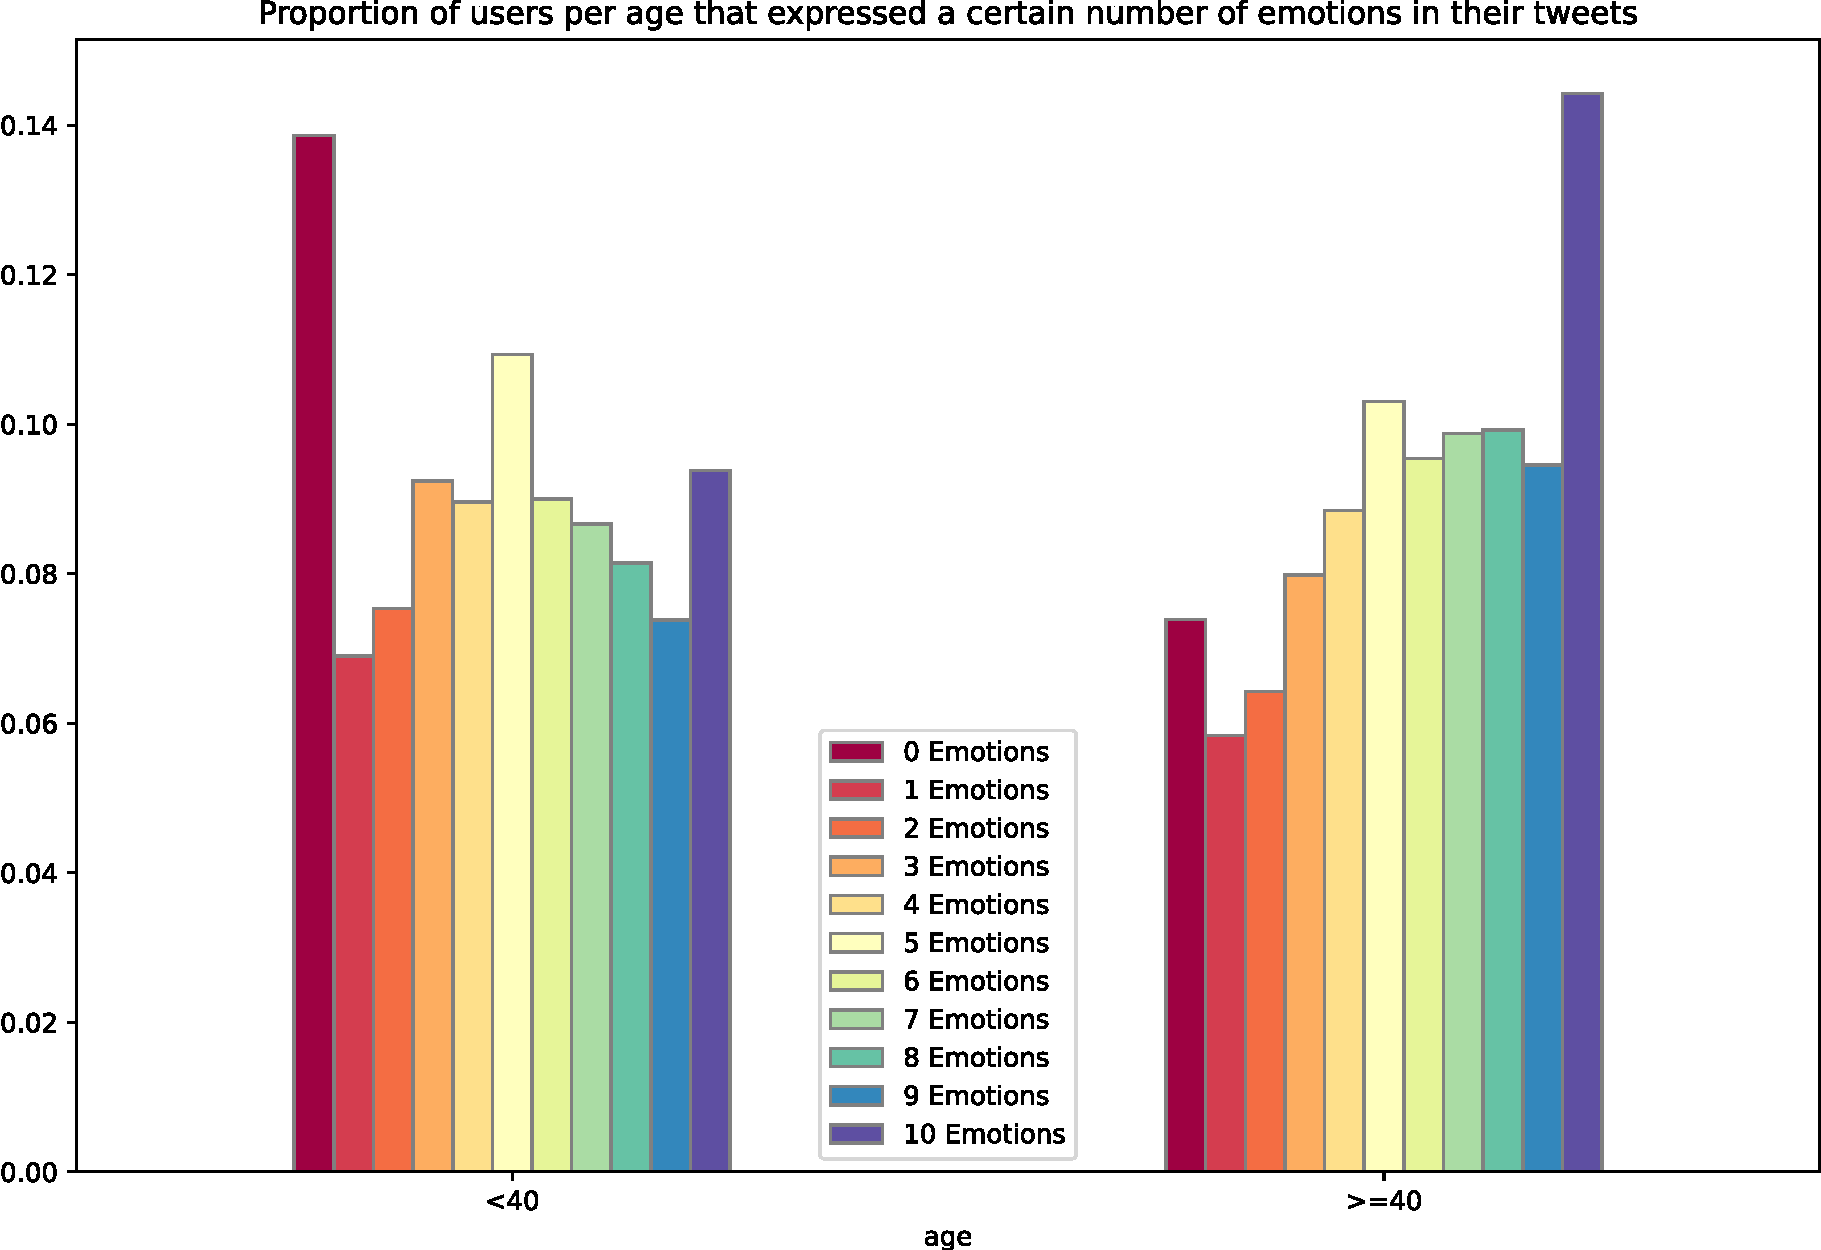
\includegraphics[scale=.25]{assets/img/en_number_of_emotions_per_age.svg.pdf}
    	\caption{Proportion of users per age expressing zero or more emotions/sentiments}
    	\label{fig:en-4-emotions-per-age-per-number}
    \end{figure}
    
\end{frame}

\begin{frame}[plain,noframenumbering]{Users per state in the Italian tweets}
    
    \begin{figure}[H]
	\centering
    	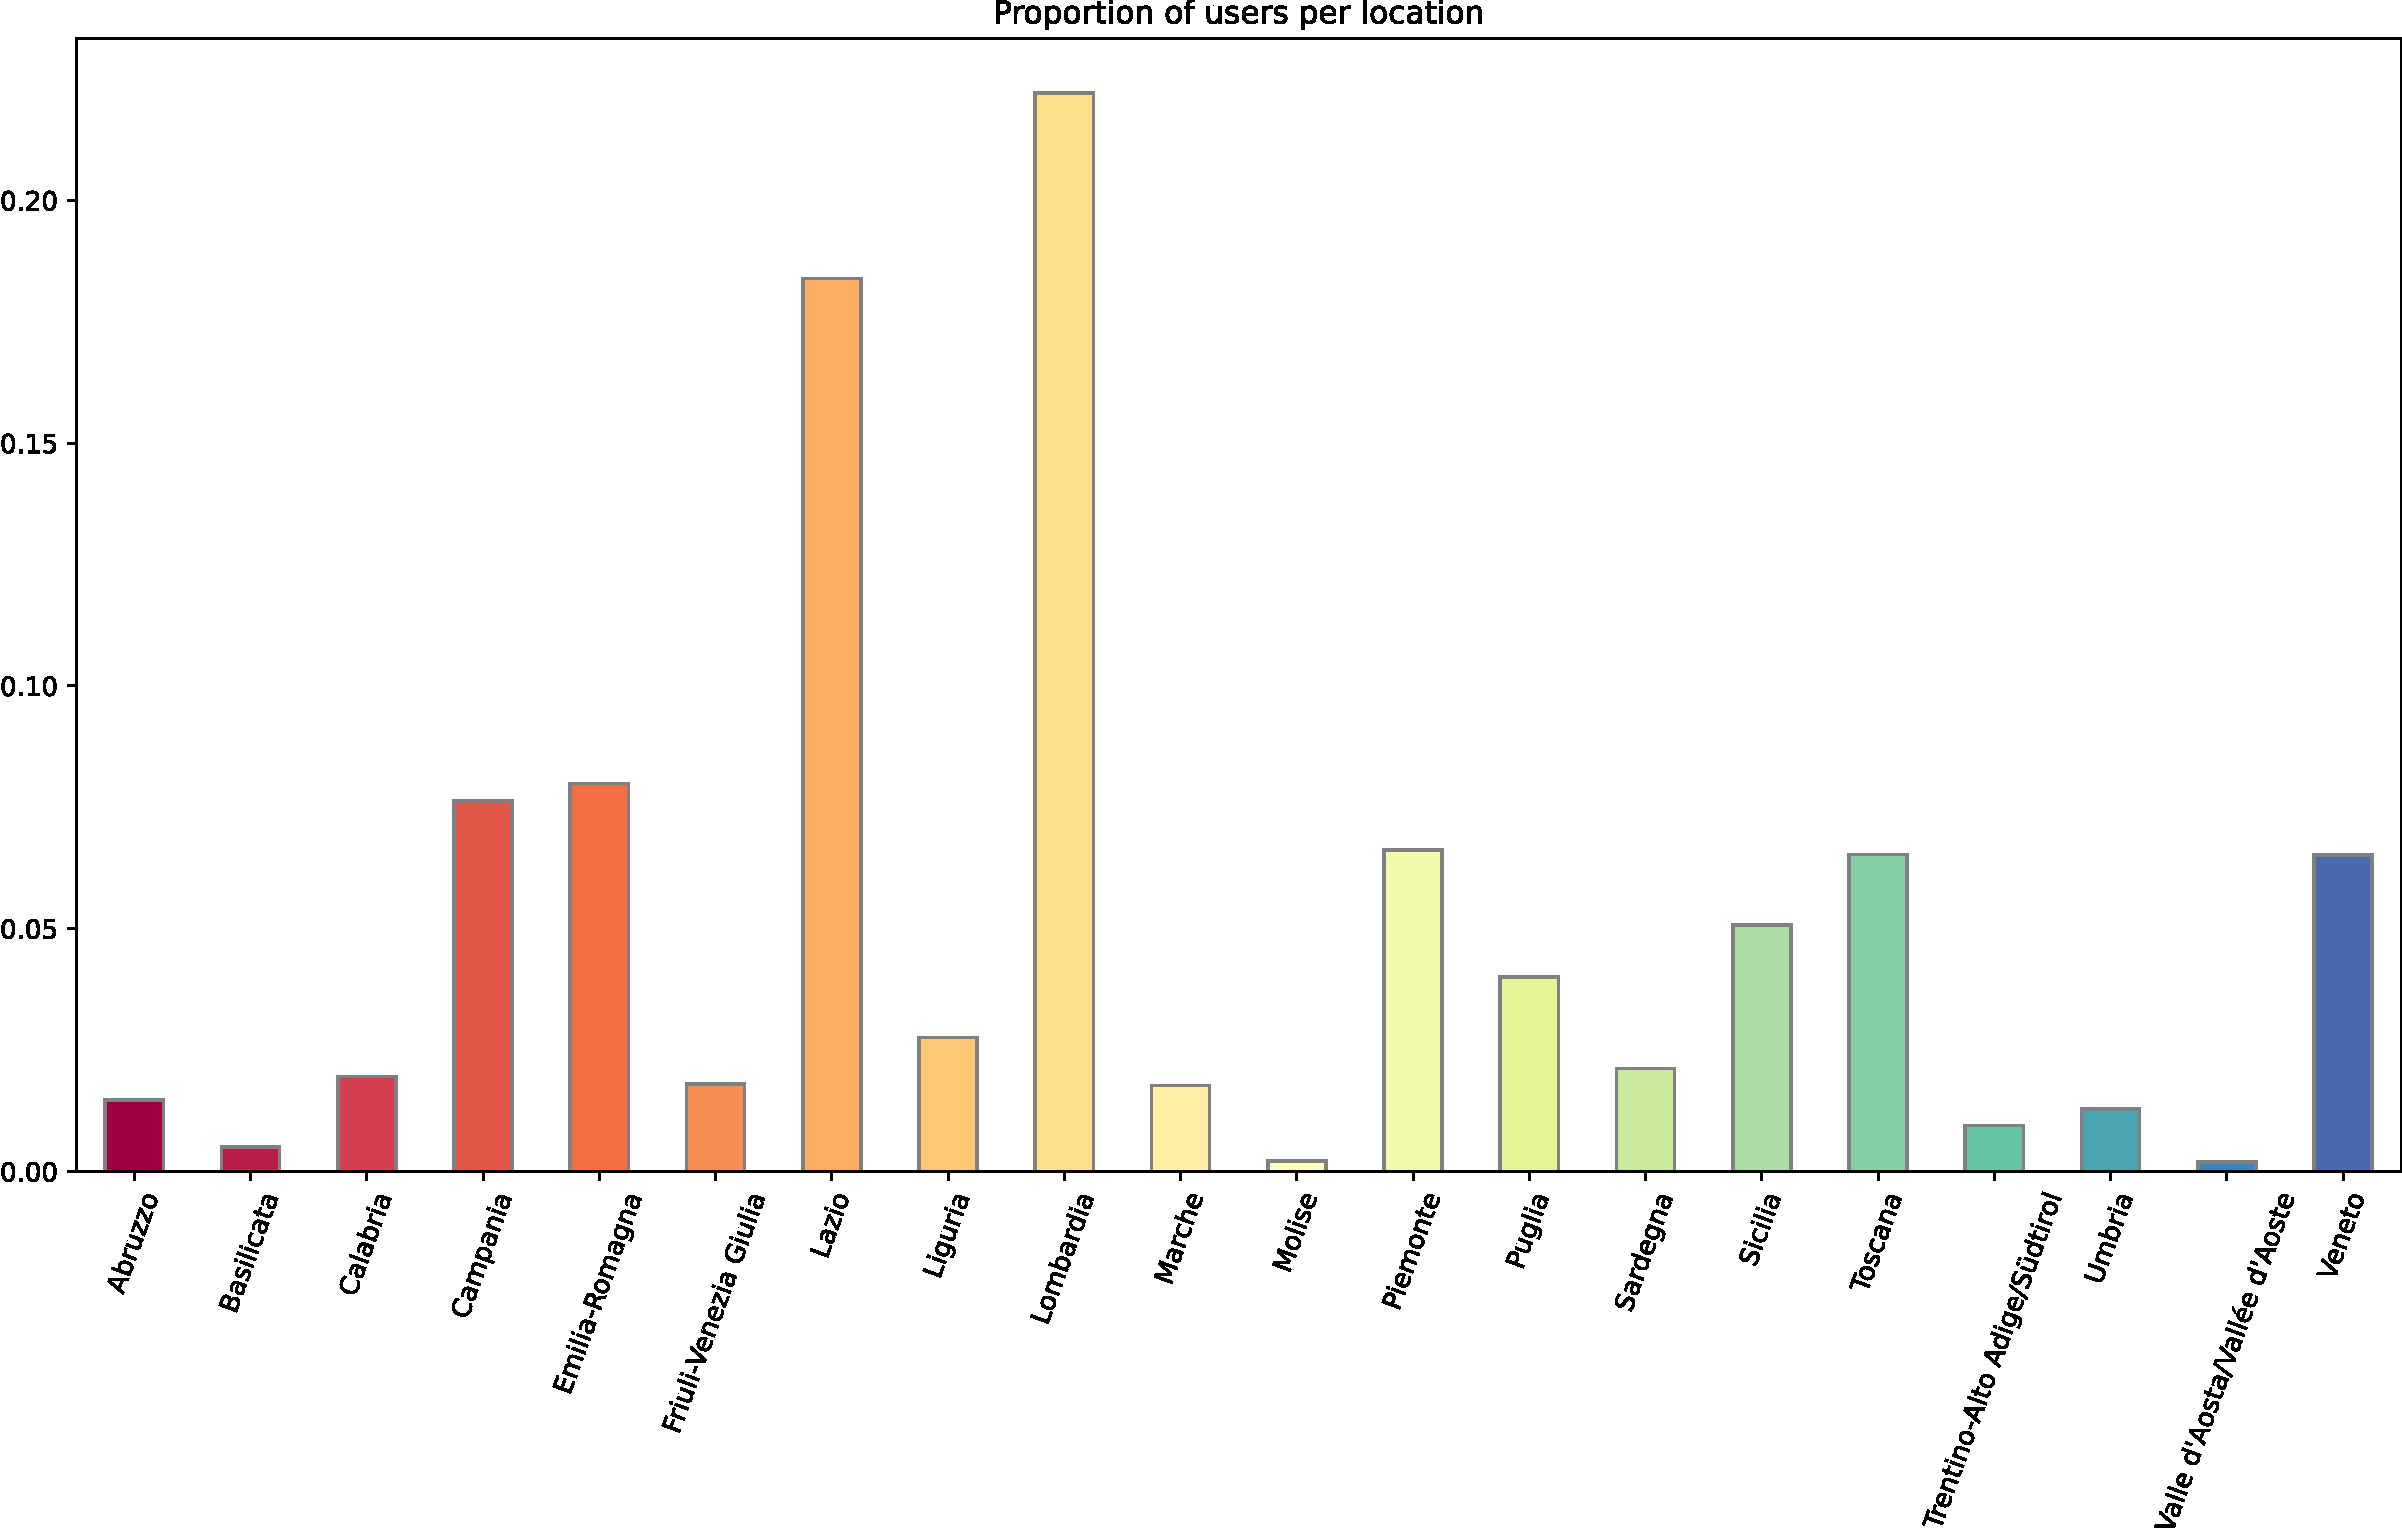
\includegraphics[scale=.25]{assets/img/it_users_per_state.svg.pdf}
    	\caption{Proportion of users per state in Italy}
    	\label{fig:it-users-state}
\end{figure}
    
\end{frame}

\begin{frame}[plain,noframenumbering]{Tweets from Campania expressing anger per week}
    
    \begin{figure}[H]
        \centering
        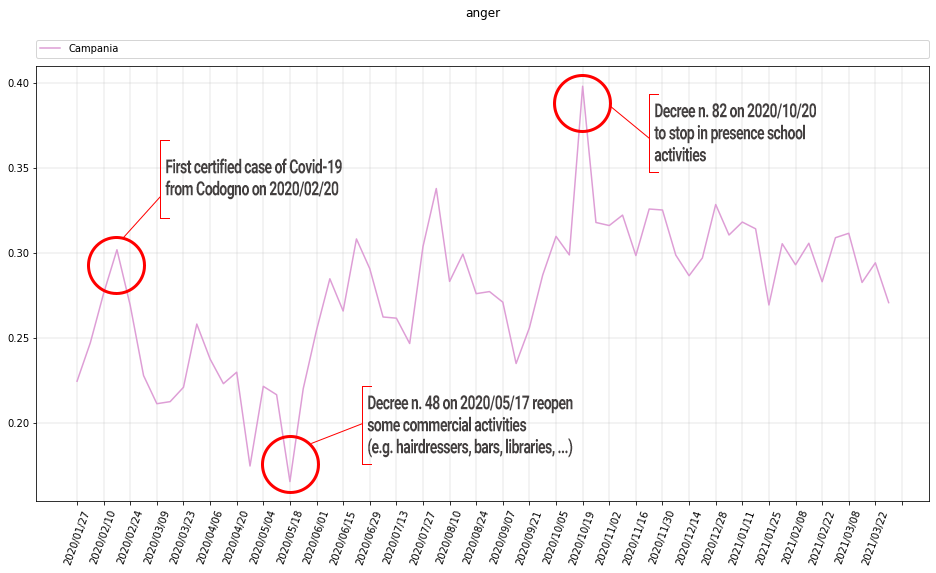
\includegraphics[scale=0.3]{assets/img/it_Campania_anger_with_events.png}
        \caption{Italian tweets from Campania expressing anger per week}
        \label{fig:it_Campania_anger}
    \end{figure}
    
\end{frame}

\begin{frame}[plain,noframenumbering]{Tweets from Campania expressing joy per week}
    
    \begin{figure}[H]
        \centering
        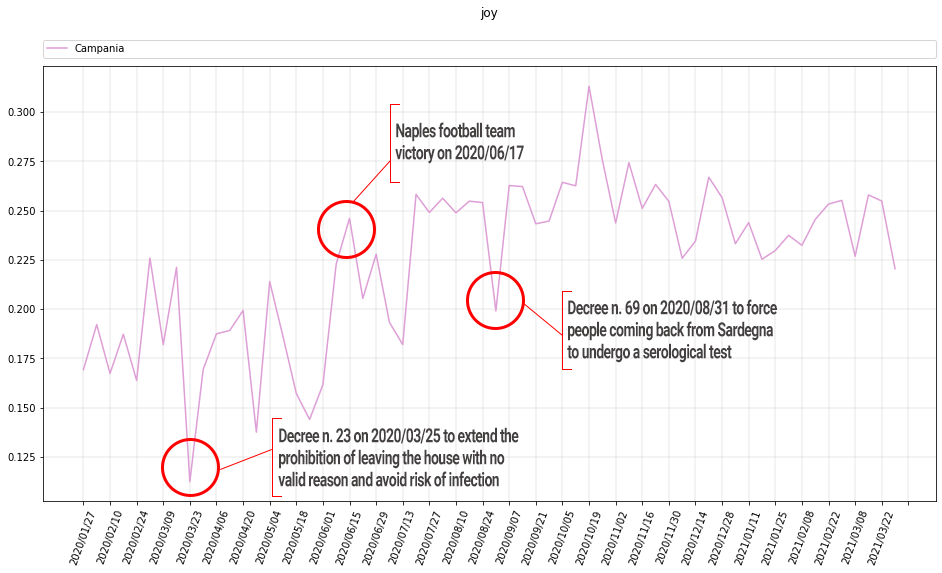
\includegraphics[scale=0.3]{assets/img/it_Campania_joy_with_events.png}
        \caption{Italian tweets from Campania expressing joy per week}
        \label{fig:it_Campania_joy}
    \end{figure}
    
\end{frame}

\end{document}
